% Please use this command sequence for proper compilation of your document
% 1) pdflatex main
% 2) makeindex main.idx -s StyleInd.ist
% 3) biber main
% 4) pdflatex main
% 5) pdflatex main


%----------------------------------------------------------------------------------------
%	PACKAGES AND OTHER DOCUMENT CONFIGURATIONS
%----------------------------------------------------------------------------------------

\documentclass[12pt, a4paper, twoside]{book}
\usepackage[top=2cm,bottom=2cm,left=2.2cm,right=2.2cm,headsep=10pt,a4paper]{geometry} % Page margins



%----------------------------------------------------------------------------------------
%	VARIOUS REQUIRED PACKAGES
%----------------------------------------------------------------------------------------
%\newcommand{\figref}[1]{\figurename~\ref{#1}}
%\newcommand{\tabref}[1]{Table~\ref{#1}}
%\newcommand{\secref}[1]{Sec.~\ref{#1}}
%\renewcommand{\eqref}[1]{Eq.~(\ref{#1})}
%
%\newcommand{\kommentar}[1]{\-\marginpar[\raggedleft\footnotesize \textsf {#1}]{\raggedright\footnotesize \textsf {#1}}}

%expected value
\newcommand{\E}[1]{\mathrm{E}{  \left(  #1 \right)  }}
\newcommand{\EY}[2]{\mathrm{E}_{#1}{  \left(  #2 \right)  }}

\newcommand{\mean}[1]{m_{#1}}
\newcommand{\autocorr}[1]{\varphi_\mathrm{#1#1}}
\newcommand{\crosscorr}[1]{\varphi_\mathrm{#1}}
\newcommand{\crosscorre}[1]{\widehat{\varphi}_\mathrm{#1}}
\newcommand{\Autocorr}[1]{\Phi_\mathrm{#1#1}}
\newcommand{\Crosscorr}[1]{\Phi_\mathrm{#1}}
\newcommand{\Autocorrbf}[1]{\boldsymbol{\Phi}_\mathrm{#1#1}}
\newcommand{\Crosscorrbf}[1]{\boldsymbol{\Phi}_\mathrm{#1}}
\newcommand{\autocorre}[1]{\widehat{\varphi}_\mathrm{#1#1}}
\newcommand{\corrvec}[1]{\mathbf{\varphi}_\mathrm{#1}}
\newcommand{\corrmat}[1]{\mathbf{R}_\mathrm{#1}}
\newcommand{\psd}[1]{\Phi_{#1}}

% function name
\newcommand{\funcname}[1]
{\mathrm{#1}}

% estimate
\newcommand{\estimation}[1]
{\ensuremath{\widehat{#1}}} % symbol for estimation

%smoothed quantity
\newcommand{\smoothB}[1]{\widetilde{#1}}
\newcommand{\smooth}[1]{\bar{#1}}

\renewcommand{\vec}[1]{\boldsymbol{#1}} % vector

% variance of ... \var{x} \sigma
\newcommand{\var}[1]{\funcname{var}\!\lefta{#1}} 
\newcommand{\cov}[1]{\mbox{cov}\!\lefta{#1}}

% e to the power of ... ( e^{} )
\newcommand{\epow}[1]{\funcname{e}^{#1}}

% argmax operator
\newcommand{\argmax}[1]{
\underset{#1}{\funcname{argmax}}}



% frequency domain
\newcommand{\numfreq}%
	{\ensuremath{N} }   		%number of samples per segment
\newcommand{\frameshift}%
	{\ensuremath{R} }	% frame shift
\newcommand{\freqi}%
	{\ensuremath{k} }   		% frequency index
\newcommand{\framei}%
	{\ensuremath{\ell} }    		% frame index
\newcommand{\ff}{_\freqi\!\lefta{\framei}} % function of (frequ,frame)
\newcommand{\ffprev}{_\freqi\!\lefta{\framei-1}} % function of (frequ,frame-1)

%real and imaginary part
\newcommand{\real}[1]{\mathrm{Re}\leftc{#1}} % Re{.}
\newcommand{\imag}[1]{\mathrm{Im}\leftc{#1}} % Im{.}



%===========================================================
%=== SIGNALS/SPECTRA
%===========================================================
\newcommand{\Xc}%  complex random variable
        {\ensuremath{X} }  % complex spectrum of speech S
\newcommand{\Xcf}%
       {\ensuremath{\Xc_\freqi} } 
\newcommand{\xrf}%
       {\ensuremath{\xr_\freqi} }
\newcommand{\xr}%
       {\ensuremath{x} }  
\newcommand{\Sc}%  complex random variable
        {\ensuremath{S} }  % complex spectrum of speech S
\newcommand{\Scf}%
       {\ensuremath{\Sc_\freqi} } 
\newcommand{\Scff}%
       {\ensuremath{\Sc\ff} } 
\newcommand{\sr} %realization
        {\ensuremath{s} }
\newcommand{\srf}%
       {\ensuremath{\sr_\freqi} } 
\newcommand{\srff}%
       {\ensuremath{\sr\ff} } 
\newcommand{\ssig}
       {\ensuremath{s[n]} }
\newcommand{\Sa}%  magnitude of complex random variable
        {\ensuremath{A} }  % 
        \newcommand{\sar}%  magnitude of complex realization
        {\ensuremath{a} }  % 
\newcommand{\Saf}%
       {\ensuremath{\Sa_\freqi} } 
\newcommand{\Saff}%
       {\ensuremath{\Sa\ff} } 
\newcommand{\Sphase}% speech phase random variable
        {\ensuremath{\Phi} }  % speech phase random variable
\newcommand{\Sphasef}% speech phase random variable
        {\ensuremath{\Sphase_\freqi} }  % speech phase random variable
 \newcommand{\sphase}% speech phase realization
        {\ensuremath{\phi} }  % speech phase realization\newcommand{\Nc}%
\newcommand{\Nc}%  complex random variable
	{\ensuremath{N} }
\newcommand{\Ncf}%
	{\ensuremath{\Nc_\freqi} }	
\newcommand{\Ncff}%
	{\ensuremath{\Nc\ff} }
\newcommand{\nr}%
	{\ensuremath{n} }
\newcommand{\nrf}%
	{\ensuremath{\nr_\freqi} }	
\newcommand{\nrff}%
	{\ensuremath{\nr\ff} } 		
\newcommand{\nsig}
       {\ensuremath{n[n]} }

\newcommand{\Yc}%
	{\ensuremath{Y} }
\newcommand{\Ycf}%
       {\ensuremath{\Yc_\freqi} } 	
\newcommand{\Ycff}%
	{\Yc\ff}
\newcommand{\yr}%
	{\ensuremath{y} }
\newcommand{\yrf}%
       {\ensuremath{\yr_\freqi} } 	
\newcommand{\yrff}%
	{\yr\ff}
\newcommand{\ysig}
       {\ensuremath{y[n]} }
\newcommand{\yframe}
       {\ensuremath{\underline{y}_\framei} }
\newcommand{\sframe}
       {\ensuremath{\underline{s}_\framei} }
\newcommand{\Ya}%  magnitude of complex random variable
        {\ensuremath{R} }  %
\newcommand{\Yaf}%  magnitude of complex random variable
        {\ensuremath{R_\freqi} }  %  
        \newcommand{\yar}%  magnitude of realization
        {\ensuremath{r} }  % 
       \newcommand{\Yphase}% noisy phase random variable
        {\ensuremath{\Theta} }  % noisy phase random variable
\newcommand{\Yphasef}% noisy phase random variable
        {\ensuremath{\Yphase_\freqi} }  % noisy phase random variable
 \newcommand{\yphase}% noisy phase realization
        {\ensuremath{\theta} }  % noisy phase realization
% Cepstrum
\newcommand{\sq}%
	{\ensuremath{s} }  	
\newcommand{\sqcf}%
	{\sq\cf}
\newcommand{\sqc}%
	{{\sq_\cepsi}}
  \newcommand{\sqtcf}%
	{\widetilde{\sq}\cf}
    \newcommand{\sqtc}%
	{\widetilde{\sq}_\cepsi}			

\newcommand{\nq}%
	{\ensuremath{n} }  	
\newcommand{\nqcf}%
	{\nq\cf}	
  \newcommand{\nqtcf}%
	{\widetilde{\nq}\cf}	
\newcommand{\nqtc}%
	{\widetilde{\yq}_\cepsi}

\newcommand{\yq}%
	{\ensuremath{y} }  	
\newcommand{\yqcf}%
	{\yq\cf}		
\newcommand{\yqtcf}%
	{\widetilde{\yq}\cf}	
\newcommand{\yqtc}%
	{\widetilde{\yq}_\cepsi}

% estimation 

\newcommand{\stime}{s}
\newcommand{\ytime}{y}
\newcommand{\ntime}{n}
\newcommand{\setime}{\widehat{s}}

\newcommand{\Sec}%
        {\ensuremath{\estimation{\Sc}} }    % estimation of S
\newcommand{\Seff}{\Sec\ff}            % estimation of S (frequ,frame)
\newcommand{\Secf}{\Sec_\freqi}            % estimation of S (frequ,frame)
\newcommand{\Seffprev}{\Sec\ffprev}            % estimation of S (frequ,frame)

\newcommand{\seff}%
        {\ensuremath{\estimation{\sr}\ff } }    % realization of estimate
\newcommand{\ssigest} %signal estimate
       {\ensuremath{\estimation{s}[n]} }
\newcommand{\sframeest}
       {\ensuremath{\estimation{\underline{s}}_\framei} }%frame estimate
\newcommand{\Saestff}%
       {\ensuremath{\estimation{\Sa}\ff} } 

\newcommand{\Saest}%
       {\ensuremath{\estimation{\Sa}} } 

%===========================================================
%=== DCT / CEPSTRUM
%===========================================================
\newcommand{\dct}[1]{\funcname{DCT}\leftc{#1}}
\newcommand{\idct}[1]{\funcname{IDCT}\leftc{#1}}
\newcommand{\cepsi}{q}
\newcommand{\cf}{_\cepsi\!\lefta{\framei}}
\newcommand{\cfprev}{_\cepsi(\framei-1)}
\newcommand{\pitch}{f_0}

%===========================================================



%===========================================================
%=== STATISTICS
%===========================================================

\newcommand{\pdfg}[2]%
	{\ensuremath{\,p_{#1}\!\!\lefta{#2}} }	% general pdf p.(.)
\newcommand{\pdfs}[1]%
    {\ensuremath{{\pdfg{s}{#1}} }}    	        % ps(.)
\newcommand{\pdfn}[1]%
    {\ensuremath{{\pdfg{n}{#1}} }}     	        % pn(.)
\newcommand{\pdf}[1]{\pdfg{\,}{#1}}      	% p(.)
% conditional pdf
\newcommand{\pdfcond}[2]{\pdf{#1\cnd#2}}
\newcommand{\pdfh}[1]{\pdfg{h}{#1}}      	% histogram

\newcommand{\sig}[1]{\sigma_{\!\scriptscriptstyle \mathrm{#1}}}%
\newcommand{\sigS}{\sigma_{\!\scriptscriptstyle \mathrm{S}}}%  deviation of speech ss
\newcommand{\sigSf}{\sigma_{\!{\scriptscriptstyle \mathrm{S}},\freqi}}% 
\newcommand{\sigSfp}{\sigma_{\!{\scriptscriptstyle \mathrm{S}},\freqi-1}}% 
\newcommand{\sigSfpp}{\sigma_{\!{\scriptscriptstyle \mathrm{S}},\freqi+1}}% 
\newcommand{\sigSsq}{\sigma^2_{\!\scriptscriptstyle \mathrm{S}}}%
\newcommand{\sigSsqf}{\sigma^2_{\!{\scriptscriptstyle \mathrm{S}},\freqi}}%  
\newcommand{\sigSsqff}{\sigma^2_{\!{\scriptscriptstyle \mathrm{S}},\freqi}(\framei)}%  
\newcommand{\sigSe}{\estimation{\sigma}_{\!{\scriptscriptstyle \mathrm{S}}}}
\newcommand{\sigSef}{\estimation{\sigma}_{\!{\scriptscriptstyle \mathrm{S}},\freqi}}% 
\newcommand{\sigSeSq}{\estimation{\sigma^2_{\!{\scriptscriptstyle \mathrm{S}}}}} % sigmaS squared estimate

\newcommand{\sigN}{\sigma_{\!\scriptscriptstyle \mathrm{N}}}% deviation of noise sn
\newcommand{\sigNf}{\sigma_{\!{\scriptscriptstyle \mathrm{N}},\freqi}}%
\newcommand{\sigNsqf}{\sigma^2_{\!{\scriptscriptstyle \mathrm{N}},\freqi}}%  
\newcommand{\sigNsq}{\sigma^2_{\!\scriptscriptstyle \mathrm{N}}}% 
\newcommand{\sigNe}{\estimation{\sigma}_{\!{\scriptscriptstyle \mathrm{N}}}}
\newcommand{\sigNef}{\estimation{\sigma}_{\!{\scriptscriptstyle \mathrm{N}},\freqi}}% 
\newcommand{\sigNeSq}{\estimation{\sigma^2_{\!{\scriptscriptstyle \mathrm{N}}}}}
\newcommand{\sigNefSq}{\estimation{\sigma^2_{\!{\scriptscriptstyle \mathrm{N}},\freqi}}}% 
\newcommand{\sigNsqff}{\sigma^2_{\!{\scriptscriptstyle \mathrm{N}},\freqi}(\framei)}%  

\newcommand{\sigXfSq}{{\sigma^2_{\!{\scriptscriptstyle \mathrm{X}},\freqi}}}% 


\newcommand{\sigY}{\sigma_{\!\scriptscriptstyle \mathrm{Y}}}% 
\newcommand{\sigYf}{\sigma_{\!{\scriptscriptstyle \mathrm{Y}},\freqi}}% 

\newcommand{\sigSsqfML}{\sigma^{2,\mathrm{ML}}_{\!\scriptscriptstyle \mathrm{S},\freqi}}%
\newcommand{\sigSsqML}{\sigma^{2,\mathrm{ML}}_{\!\scriptscriptstyle \mathrm{S}}}%        

\newcommand{\sigSefSq}{\estimation{\sigma^2_{\!{\scriptscriptstyle \mathrm{S}},\freqi}}}% 

                                        
\newcommand{\prob}[1]{P\!\lefta{#1}}  % probability P(.)
\newcommand{\probc}[2]{P\!\lefta{#1 \cnd #2}}
\newcommand{\probcRV}[4]{P_{#1 \mid #2}\!\lefta{#3 \mid #4}}
                                        % conditional probability P(.)
\newcommand{\cnd}{\bigm|}               % condition |

\newcommand{\hyp}[1]{{\cal H}_{#1}}     % hypothesis
\newcommand{\hypf}[1]{{\cal H}_{#1,\freqi}}     % hypothesis
\newcommand{\hypff}[1]{{\cal H}_{#1,\freqi}(\framei)}     % hypothesis

\newcommand{\est}[1]{E\leftc{#1}}       % estimate E{.}
\newcommand{\estc}[2]{E\leftc{\left.#1\right|#2}}
                                % conditional estimate E{.|.}
\newcommand{\varc}[2]{\,\mbox{\it Var}\leftc{\left.#1\right|#2}}
                                % conditional variance Var{.|.}

%===========================================================
%=== SNR
%===========================================================
\newcommand{\snr}%
    {\ensuremath{\xi} }% a priori SNR
\newcommand{\snrf}%
    {\ensuremath{\snr_\freqi} }%     
\newcommand{\snrff}%
    {\ensuremath{\snr\ff} }% 

\newcommand{\snrg}[1]{\snr_{#1}}% general 
\newcommand{\snrmin}{\snrg{\mathrm{min}}}% 

\newcommand{\snre}{\estimation{\snr}}% estimated a priori SNR
\newcommand{\snreff}{\snre\ff}% 
\newcommand{\snrefprev}{\snre\ffprev}% 
                                    % (frequ,frame-1)

\newcommand{\snrpost}{\zeta} % aposteriori SNR
\newcommand{\snrpostRV}{Z} % random variable: HERE WE NEED ANOTHER NAME
\newcommand{\snrpostRVf}{Z_\mathrm{\freqi}} % random variable: HERE WE NEED ANOTHER NAME
\newcommand{\snrpostf}{\snrpost_\freqi}
\newcommand{\snrpostff}{\snrpost\ff}
\newcommand{\snrposte}{\estimation{\snrpost}}
\newcommand{\snrpostef}{\estimation{\snrpost}_\freqi}
\newcommand{\snrposteff}{\estimation{\snrpost}\ff}

\newcommand{\snrpostth}{{\snrpost_{th}}}

\newcommand{\segimp}{\Delta\segsnr} % improvement of seg. SNR

%===========================================================
%=== FUNCTIONS
%===========================================================
\newcommand{\gain}{g}
\newcommand{\Gain}{G}
\newcommand{\Gainf}{\Gain_\freqi}
\newcommand{\Gainff}{\Gain\ff}
\newcommand{\Gainhypf}[1]{\Gain_{\hypnof{#1},\freqi}}
\newcommand{\Gainmin}{\Gain_{\mb{min}}}
\newcommand{\Gainlim}{\widetilde{\Gain}}
\newcommand{\Gainlimf}{{\widetilde{\Gain}_\freqi}}


\newcommand{\segsnr}%
	{\ensuremath{\funcname{SNR}_{seg}} }% segmental SNR
\newcommand{\mos}{MOS}% Mean-Opinion Score value

%===========================================================
%=== BRACKETS
%===========================================================
\newcommand{\lefta}[1]{\left(#1\right)}
\newcommand{\leftb}[1]{\left[#1\right]}
\newcommand{\leftc}[1]{\left\{#1\right\}}


%===========================================================
%=== OPERATORS
%===========================================================

\newcommand{\erf}{\funcname{erf}}
\newcommand{\erfa}[1]{\,\mbox{erf}\!\lefta{#1}}
\newcommand{\erfi}[1]{\,\mbox{erfi}\!\lefta{#1}}
\newcommand{\erfca}[1]{\,\mbox{erfc}\!\lefta{#1}}
\renewcommand{\exp}{\funcname{exp}} 
\newcommand{\expa}[1]{\exp\!\lefta{#1}} 
\newcommand{\expb}[1]{\exp\!\leftb{#1}}    
\newcommand{\expc}[1]{\exp\!\leftc{#1}}
\newcommand{\expp}[1]{\mathrm{e}^{#1}}
\newcommand{\loga}[1]{\,\funcname{log}\!\lefta{#1}}
\newcommand{\loge}[1]{\,\funcname{log}\!\lefta{#1}}
\newcommand{\logd}[1]{\,\funcname{log}_2\!\lefta{#1}}
\newcommand{\logt}[1]{\log_{10}\!\lefta{#1}}
\newcommand{\logta}[1]{\logt\lefta{#1}}
\newcommand{\gammaf}[1]{\,\Gamma\!\lefta{#1}}% gamma function
\newcommand{\abs}[1]{\left|#1\right|}
\newcommand{\sgn}[1]{\,\mbox{sgn}\!\left(#1\right)}
\renewcommand{\jmath}{\mathrm{j}}
\newcommand{\maxa}[1]{\max\!\lefta{#1}}
\newcommand{\mina}[1]{\min\!\lefta{#1}}


\newcommand{\idftexp}[3]{1/\numfreq \sum_{#2 =0 }^{\numfreq-1} #3 \, \expp{\jmath 2\pi #2 #1 /\numfreq}}
\newcommand{\dftexp}[3]{            \sum_{#2 =0 }^{\numfreq-1} #3 \, \expp{- \jmath 2\pi #1 #2 /\numfreq}}
\newcommand{\dft}[1]%
	{\ensuremath{\funcname{DFT}\!\leftc{#1} }} %_{\dftlength}} }
	% DFT transform symbol DFT{.}_M
\newcommand{\idft}[1]%
	{\ensuremath{\funcname{IDFT}\!\leftc{#1}} } %_{\dftlength}} }

\newcommand{\intinf}{\int\limits_{-\infty}^{+\infty}}
\newcommand{\Euler}{\mbox{  \boldmath$C$}}


%===========================================================
%=== possible italics
%===========================================================
\newcommand{\apriori}{\emph{a priori }}
\newcommand{\Apriori}{\emph{A priori }}
\newcommand{\aposteriori}{\emph{a posteriori }}
\newcommand{\Aposteriori}{\emph{A posteriori }}
\newcommand{\eg}{{e.g.\ }}
\newcommand{\ie}{{i.e. }}
\newcommand{\etal}{{et~al. }}



%===========================================================
%=== units
%===========================================================
\newcommand{\ms}{\,\mathrm{ms}}
\newcommand{\Hz}{\,\mathrm{Hz}}
\newcommand{\kHz}{\,\mathrm{kHz}}

% decibel
\newcommand{\dB}{\,\mathrm{dB}}


%speech Enhancement
\newcommand{\absfshift}{L}

\newcommand{\biascorr}{\mathcal{B}}
\newcommand{\indicator}{b}

\newcommand{\alphadd}{\alpha_{\mathrm{dd}}}

\newcommand{\srate}{f_\mathrm{s}}
\newcommand{\lag}{\lambda}
\newcommand{\timei}{n}
\newcommand{\timeiseg}{\timei}
\newcommand{\alttime}{m}
\newcommand{\orderq}{q}
\newcommand{\orderp}{p}
\newcommand{\expjO}{\expp{\jmath \Omega} }



% SPP
\newcommand{\aprioriSPP}{\prob{\hyp{1}}}%{\rho}
\newcommand{\aprioriSPPhat}{\widehat{P}(\hyp{1})}
\newcommand{\aprioriSPPhatf}{\widehat{P}(\hypf{1})}
\newcommand{\aprioriSPPhatff}{\widehat{P}(\hypf{1}(\framei))}
\newcommand{\aprioriSAP}{\prob{\hyp{0}}}
% \newcommand{\apostSPP}{{\mathcal{P}_\freqi}}
\newcommand{\apostSPP}{\probc{\hyp{1}}{\Yc}}
\newcommand{\apostSPPRV}{\probcRV{\hyp{1}}{\Yc}{\hyp{1}}{\yc}}
\newcommand{\apostSPPff}{\probc{\hyp{1}}{\Ycff}}
\newcommand{\apostSPPfr}{\probc{\hyp{1}}{\Yc(\framei)}}
\newcommand{\apostP}{\mathcal{P}}
\newcommand{\apostSAP}{{\probc{\hyp{0}}{y}}}
\newcommand{\apostSAPf}{\apostSAP}



\newcommand{\Per}{\mathrm{Per}}
\newcommand{\Perf}{\mathrm{Per}_\freqi}
\newcommand{\per}{\mathrm{per}}
\newcommand{\perf}{\mathrm{per}_\freqi}


\newcommand{\samplingPeriod}{T_{s}}
\newcommand{\samplingFreq}{f_{s}}
\newcommand{\sampTime}{t}
\newcommand{\sampIndex}{n}
\newcommand{\fourierSym}{\mathfrak{F}}
\newcommand{\deltaPulse}{\delta}
\newcommand{\contFunc}{x}
\newcommand{\discFunc}{d}
\newcommand{\sinCoef}{a}
\newcommand{\cosCoef}{b}




%--- from PPre format
\usepackage[dvips]{graphicx}            % für zwei Bilder in Pelton Versuch
%\usepackage{graphicx}                   % neue Graphik Umgebung
\usepackage{color}
% \usepackage{epsfig}                   % war mal ... 
\usepackage{wrapfig}                    % JJT: for wrapping text around figs.
\usepackage{floatflt}                      % wof"ur? - irgendwas f"ur ToC
\usepackage{fancyhdr}                   % f�r all die Kopf- & Fu�zeilen
\usepackage{german}                     % Grundeinstellungen
\usepackage{times,a4wide}
% \usepackage[applemac]{inputenc}        % Umlaute von Tastatur
% \usepackage[microsoft]{inputenc}       % Umlaute von Tastatur
\usepackage{setspace}                   % f"ur `doublespacing' z.B.
\usepackage{versions}                    % `comments' u.�.
%\usepackage{indentfirst}               % auch erster Absatz erh"alt Einzug
%\usepackage{latexsym,ae}
\usepackage{verbatim}
%\usepackage{babel}
\usepackage[section] {placeins}					%to (hopefully) avoid too many unprocessed floats
\usepackage{epic}                       % f�r Spektrum Skizze
                                        %       -- mu� vor pictex stehen
%%%%%%%\usepackage{pictex}                     % l"adt `pictex' f"ur einige Pumpen Bilder
                                        % `pictexwd' ist verbessertes Modul,
                                        % l"auft aber nicht auf Mac, uk
\usepackage[squaren]{SIunits}           % /metre u.a. im mathematikmodus

\usepackage[latin9]{inputenc}		% für die Umlaute von Tastatur

%\renewcommand{\familydefault}{\sfdefault} %Set default font to sans serif 
		
\selectlanguage{english}            % Hauptsprache: britisches Englisch

\newcommand{\version}{30.09.07}    % damit etwas in der Variablen steht ...
\newcommand{\name}[1]{\textsc{#1}}
%--- /from PPre format

\usepackage{titlesec} % Allows customization of titles


%\titleformat{\part}[block]{\normalfont\sffamily}{}{}{}{} %/rk:doesn't work just like this

\usepackage[T1]{fontenc}
%\usepackage[latin1]{inputenc} %wird in format_PPRE_reader definiert
%\usepackage{graphicx} % wird in format_PPRE_reader definiert

\usepackage{xcolor} % Required for specifying colors by name
\definecolor{chapcolor}{RGB}{243,102,25} % Define the orange color used for highlighting throughout the book

% Font Settings
\usepackage{avant} % Use the Avantgarde font for headings


\usepackage{graphicx} % Required for including pictures

\usepackage{lipsum} % Inserts dummy text

\usepackage{tikz} % Required for drawing custom shapes
\usetikzlibrary{arrows,calc,positioning}
%\usepackage{subfig}

\usepackage{pgfplots} % Required for drawing custom shapes
\pgfplotsset{width=7cm,compat=1.8}
%a) add the path to the /bin directory where u installed gnuplot to the windows "path" variable (und%er control panel -> system -> advanced -> environment variables)
%b) make sure there is a COPY of the executable in the /bin folder called "gnuplot.exe" (what i had to do is copy "pgnuplot.exe" to "gnuplot.exe"... wtf!?)
%c) add "-enable-write18" to the command line options of the output profile ur using in texniccenter

\usepackage[labelfont=bf,textfont=small]{caption}
% will apply to all subcaptions
\usepackage[labelfont=bf,textfont=small,singlelinecheck=on,justification=raggedright]{subcaption}

\usepackage[english]{babel} % English language/hyphenation

\usepackage{enumitem} % Customize lists
\setlist{nolistsep} % Reduce spacing between bullet points and numbered lists

\usepackage{booktabs} % Required for nicer horizontal rules in tables

\usepackage{eso-pic} % Required for specifying an image background in the title page

\usepackage{floatrow} % Required for setting the captions beside the image in a figure environment, generates error with double captions

%Bibliograhy packages
\usepackage{csquotes} %Required by bibtex
% \usepackage[style=alphabetic, bibstyle=alphabetic, backend=biber]{biblatex}
% \usepackage[nottoc, section, numbib, numindex]{tocbibind}  % fuegt
\usepackage[nottoc, numbib, numindex]{tocbibind}  % fuegt Literaturverzeichnis ins Inhaltsverzeichnis ein

\usepackage[colorlinks=true,
linkcolor=black,
citecolor=black,
filecolor=black,
urlcolor=black,
bookmarks=true,
bookmarksopen=true,
bookmarksopenlevel=1,
plainpages=false,
pdfpagelabels=true]{hyperref} %rereferencing


 \DeclareFontFamily{U}{wncy}{}
    \DeclareFontShape{U}{wncy}{m}{n}{<->wncyr10}{}
    \DeclareSymbolFont{mcy}{U}{wncy}{m}{n}
    \DeclareMathSymbol{\Sh}{\mathord}{mcy}{"58} 



% Index
\usepackage{calc} % For simpler calculation - used for spacing the index letter headings correctly
\usepackage{makeidx} % Required to make an index
\makeindex % Tells LaTeX to create the files required for indexing

% Define box and box title style
\tikzstyle{mybox} = [draw=red, fill=blue!20, very thick,
    rectangle, rounded corners, inner sep=0.25\linewidth, inner ysep=10pt]
\tikzstyle{fancytitle} =[fill=red, text=white]

%Remove Part before Apendix
%\renewcommand{\partname}{}

%\usepackage{morefloats}  % damit mehr floating  graphics verarbeitet werden k�nnen
%----------------------------------------------------------------------------------------
%	MAIN TABLE OF CONTENTS
%----------------------------------------------------------------------------------------

\usepackage{titletoc} % Required for manipulating the table of contents

\contentsmargin{0cm} % Removes the default margin

% Part text styling
\titlecontents{part}[1.25cm] % Indentation
{\addvspace{15pt}\large\sffamily\bfseries} % Spacing and font options for chapters
{\color{black!60}\contentslabel[\Large\thecontentslabel]{1.25cm}\color{black}} % Chapter number
{}  
{\color{black!60}\normalsize\sffamily\bfseries\;\titlerule*[.5pc]{.}\;\thecontentspage} % Page number

% Chapter text styling
%\titlecontents{chapter}[1.25cm] % Indentation
\titlecontents{chapter}[0.35cm] % Indentation
{\addvspace{15pt}\large\sffamily\bfseries} % Spacing and font options for chapters
{\color{chapcolor!60}\contentslabel[\Large\thecontentslabel]{1.25cm}\color{chapcolor}} % Chapter number
{}  
{\color{chapcolor!60}\normalsize\sffamily\bfseries\;\titlerule*[.5pc]{.}\;\thecontentspage} % Page number
% Section text styling
\titlecontents{section}[1.25cm] % Indentation
{\addvspace{5pt}\sffamily\bfseries} % Spacing and font options for sections
{\contentslabel[\thecontentslabel]{1.25cm}} % Section number
{}
{\sffamily\hfill\color{black}\thecontentspage} % Page number
[]
% Subsection text styling
\titlecontents{subsection}[1.25cm] % Indentation
{\addvspace{1pt}\sffamily\small} % Spacing and font options for subsections
{\contentslabel[\thecontentslabel]{1.25cm}} % Subsection number
{}
{\sffamily\;\titlerule*[.5pc]{.}\;\thecontentspage} % Page number
[] 

%----------------------------------------------------------------------------------------
%	MINI TABLE OF CONTENTS IN CHAPTER HEADS
%----------------------------------------------------------------------------------------

% Section text styling
\titlecontents{lsection}[0em] % Indendating
{\footnotesize\sffamily} % Font settings
{}
{}
{}

% Subsection text styling
\titlecontents{lsubsection}[.5em] % Indentation
{\normalfont\footnotesize\sffamily} % Font settings
{}
{}
{}
 
%----------------------------------------------------------------------------------------
%	PAGE HEADERS
%----------------------------------------------------------------------------------------

\usepackage{fancyhdr} % Required for header and footer configuration

\pagestyle{fancy}
\renewcommand{\chaptermark}[1]{\markboth{\sffamily\normalsize\bfseries #1}{}} % Chapter text font settings
\renewcommand{\sectionmark}[1]{\markright{\sffamily\normalsize\thesection\hspace{5pt}#1}{}} % Section text font settings
\fancyhf{}
\fancyhead[LO]{\rightmark} % Print the nearest section name on the left side of odd pages
\fancyhead[RE]{\leftmark} % Print the current chapter name on the right side of even pages
\renewcommand{\headrulewidth}{0.5pt} % Width of the rule under the header %
\addtolength{\headheight}{2.5pt} % Increase the spacing around the header slightly
\fancypagestyle{plain}{\fancyhead{}\renewcommand{\headrulewidth}{0pt}} % Style for when a plain pagestyle is specified
\fancyheadoffset{1cm}

% Removes the header from odd empty pages at the end of chapters
\makeatletter
\renewcommand{\cleardoublepage}{
\clearpage\ifodd\c@page\else
\hbox{}
\vspace*{\fill}
\thispagestyle{empty}
\newpage
\fi}

 \fancyfoot[LE,RO]{\sffamily\normalsize\thepage} % Font setting for the page number in the header
\renewcommand{\footrulewidth}{0.0pt} % Width of the rule above the footer %
\setlength{\footskip}{20mm}% Increase the spacing around the header slightly 



\fancyfoot[LO]{\sffamily\normalsize\bfseries Digital Speech Processing} % Print the nearest section name on the left side of odd pages
\fancyfoot[RE]{\sffamily\normalsize\bfseries Digital Speech Processing} % Print the current chapter name on the right side of even pages



\fancyfootoffset{1cm}%Lengthens the rule%

\setlength{\textheight}{235mm}% Increase the spacing around the header slightly 

%----------------------------------------------------------------------------------------
%	THEOREM STYLES
%----------------------------------------------------------------------------------------

\usepackage{mathtools,amsfonts,amssymb,amsthm} % For including math equations, theorems, symbols, etc

\newcommand{\intoo}[2]{\mathopen{]}#1\,;#2\mathclose{[}}
\newcommand{\ud}{\mathop{\mathrm{{}d}}\mathopen{}}
\newcommand{\intff}[2]{\mathopen{[}#1\,;#2\mathclose{]}}
\newtheorem{notation}{Notation}[chapter]

\newtheoremstyle{chapcolornum} % Theorem style name
{7pt} % Space above
{7pt} % Space below
{\normalfont} % Body font
{} % Indent amount
{\small\bf\sffamily\color{chapcolor}} % Theorem head font
{\;\;} % Punctuation after theorem head
{0.25em} % Space after theorem head
{\small\sffamily\color{chapcolor}\thmname{#1}
%{\small\sffamily\color{chapcolor}\thmname{#1}\thmnumber{\@ifnotempty{#1}{ }\@upn{#2}} % Theorem text (e.g. Theorem 2.1)
\thmnote{\ {\the\thm@notefont\sffamily\bfseries\color{black}--- #3.}}} % Optional theorem note
\renewcommand{\qedsymbol}{$\blacksquare$} % Optional qed square

\newtheoremstyle{blacknumex} % Theorem style name
{7pt} % Space above
{7pt} % Space below
{\normalfont} % Body font
{} % Indent amount
{\small\bf\sffamily} % Theorem head font
{\;\;} % Punctuation after theorem head
{0.25em} % Space after theorem head
%{\small\sffamily{\tiny\ensuremath{\blacksquare}}\ \thmname{#1}\thmnumber{\@ifnotempty{#1}{ }\@upn{#2}} % Theorem text (e.g. Theorem 2.1) %Removed black qed box in next line
{\ \thmname{#1}\thmnumber{\@ifnotempty{#1}{ }\@upn{#2}} % Theorem text (e.g. Theorem 2.1)

\thmnote{\ {\the\thm@notefont\sffamily\bfseries--- #3.}}} % Optional theorem note

\newtheoremstyle{blacknum} % Theorem style name
{7pt} % Space above
{7pt} % Space below
{\normalfont} % Body font
{} % Indent amount
{\small\bf\sffamily} % Theorem head font
{\;\;} % Punctuation after theorem head
{0.25em} % Space after theorem head
{\small\sffamily\thmname{#1}\thmnumber{\@ifnotempty{#1}{ }\@upn{#2}} % Theorem text (e.g. Theorem 2.1)
\thmnote{\ {\the\thm@notefont\sffamily\bfseries--- #3.}}} % Optional theorem note

\newtheoremstyle{nonum} % Theorem style name
{7pt} % Space above
{7pt} % Space below
{\normalfont} % Body font
{} % Indent amount
{\small\bf\sffamily} % Theorem head font
{\;\;} % Punctuation after theorem head
{0.25em} % Space after theorem head
{\small\sffamily\thmname{#1} % Theorem text (e.g. Theorem 2.1)
\thmnote{\ {\the\thm@notefont\sffamily\bfseries--- #3.}}} % Optional theorem note

\makeatother


% Defines the theorem text style for each type of theorem to one of the three styles above
\theoremstyle{chapcolornum}
%\newtheorem{theoremeT}{Theorem}[chapter]
\newtheorem{theoremeT}{Important}
\newtheorem{proposition}{Proposition}[chapter]
\newtheorem{problem}{Problem}[chapter]
\newtheorem{exerciseT}{Exercise}[chapter]
\theoremstyle{blacknumex}
\newtheorem{exampleT}{Example}[chapter]
\theoremstyle{blacknum}
\newtheorem{vocabulary}{Vocabulary}[chapter]
\newtheorem{definitionT}{Definition}[chapter]
\theoremstyle{nonum}
\newtheorem{corollaryT}{Learning objectives}



%----------------------------------------------------------------------------------------
%	DEFINITION OF COLORED BOXES
%----------------------------------------------------------------------------------------

\RequirePackage[framemethod=default]{mdframed} % Required for creating the theorem, definition, exercise and corollary boxes

% Theorem box
\newmdenv[skipabove=7pt,
skipbelow=7pt,
rightline=true,
leftline=true,
topline=true,
bottomline=true,
backgroundcolor=chapcolor!10,
linecolor=chapcolor,
innerleftmargin=5pt,
innerrightmargin=5pt,
innertopmargin=5pt,
innerbottommargin=5pt,
leftmargin=0cm,
rightmargin=0cm,
linewidth=1pt]{tBox}	



% Exercise box	  
\newmdenv[skipabove=7pt,
skipbelow=7pt,
rightline=false,
leftline=true,
topline=false,
bottomline=false,
backgroundcolor=chapcolor!10,
linecolor=chapcolor,
innerleftmargin=5pt,
innerrightmargin=5pt,
innertopmargin=5pt,
innerbottommargin=5pt,
leftmargin=0cm,
rightmargin=0cm,
linewidth=4pt]{eBox}	


% Definition box
\newmdenv[skipabove=10pt,
skipbelow=10pt,
rightline=false,
leftline=true,
topline=false,
bottomline=false,
linecolor=chapcolor,
innerleftmargin=5pt,
innerrightmargin=5pt,
innertopmargin=0pt,
leftmargin=0cm,
rightmargin=0cm,
linewidth=2pt,
innerbottommargin=0pt]{dBox}	

% Corollary box
\newmdenv[skipabove=7pt,
skipbelow=7pt,
rightline=false,
leftline=true,
topline=false,
bottomline=false,
linecolor=gray,
backgroundcolor=chapcolor!10,
innerleftmargin=5pt,
innerrightmargin=5pt,
innertopmargin=5pt,
leftmargin=0cm,
rightmargin=0cm,
linewidth=4pt,
innerbottommargin=5pt]{cBox}				  
		  

% Creates an environment for each type of theorem and assigns it a theorem text style from the "Theorem Styles" section above and a colored box from above
\newenvironment{theorem}{\begin{tBox}\begin{theoremeT}}{\end{theoremeT}\end{tBox}}
%\newenvironment{exercise}{\begin{eBox}\begin{exerciseT}}{\hfill{\color{chapcolor}\tiny\ensuremath{\blacksquare}}\end{exerciseT}\end{eBox}}				   %Removed black qed box in next line
\newenvironment{exercise}{\begin{eBox}\begin{exerciseT}}{\hfill{\color{chapcolor}}\end{exerciseT}\end{eBox}}
\newenvironment{definition}{\begin{dBox}\begin{definitionT}}{\end{definitionT}\end{dBox}}	
%\newenvironment{example}{\begin{exampleT}}{\hfill{\tiny\ensuremath{\blacksquare}}\end{exampleT}}		%Removed black qed box in next line
\newenvironment{example}{\begin{exampleT}}{\hfill{}\end{exampleT}}		
\newenvironment{corollary}{\begin{cBox}\begin{corollaryT}}{\end{corollaryT}\end{cBox}}	

%----------------------------------------------------------------------------------------
%	WARNING ENVIRONMENT
%----------------------------------------------------------------------------------------

\newenvironment{warning}{\par\vskip10pt\small % Vertical white space above the remark and smaller font size
\begin{list}{}{
\leftmargin=40pt % Indentation on the left
\rightmargin=25pt}\item\ignorespaces % Indentation on the right
\makebox[-2.5pt]{

 

\begin{tikzpicture}[overlay]
%\node[draw=chapcolor!60,line width=1pt,circle,fill=chapcolor!25,font=\sffamily\bfseries,inner sep=2pt,outer sep=0pt] at (-15pt,0pt){\textcolor{chapcolor}{R}};
  \node[anchor= north west] at (-40pt,15pt){\includegraphics[scale=0.45]{./Pictures/Icon_Stop/Icon-Stop.pdf} 
		}; %Semicolon important, separates icon from text
\end{tikzpicture}
} 
\advance\baselineskip -1pt}{\end{list}\vskip5pt} % Tighter line spacing and white space after remark

%----------------------------------------------------------------------------------------
%	IDEA ENVIRONMENT
%----------------------------------------------------------------------------------------

\newenvironment{idea}{\par\vskip10pt\small % Vertical white space above the remark and smaller font size
\begin{list}{}{
\leftmargin=35pt % Indentation on the left
\rightmargin=25pt}\item\ignorespaces % Indentation on the right
\makebox[-2.5pt]{

 

\begin{tikzpicture}[overlay]
%\node[draw=chapcolor!60,line width=1pt,circle,fill=chapcolor!25,font=\sffamily\bfseries,inner sep=2pt,outer sep=0pt] at (-15pt,0pt){\textcolor{chapcolor}{R}};
  \node[anchor= north] at (-15pt,0pt){\includegraphics[scale=1]{./Pictures/Icon_Idea/Idea-icon.pdf} 
		}; %Semicolon important, separates icon from text
\end{tikzpicture}
} 
\advance\baselineskip -1pt}{\end{list}\vskip5pt} % Tighter line spacing and white space after remark


%----------------------------------------------------------------------------------------
%	SECTION NUMBERING IN THE MARGIN
%----------------------------------------------------------------------------------------

\newcommand\numb[1]{{%
\begin{center}
\begin{tikzpicture}
\node (0,0) [rounded corners=25pt,fill=white,fill opacity=.6,text opacity=1,draw=chapcolor,draw opacity=1,line width=2pt,inner sep=15pt,align=
center]{\thesection \  \\ \makebox[15cm]{#1}};
\end{tikzpicture}
\end{center}
}}%

\titleformat{\section}[display]{\color{black}\normalfont\sffamily\bfseries\large}{}{0cm}{\numb}
\titlespacing{\section}{0pt}{0pt}{0pt}


\makeatletter
\renewcommand{\subsection}{\@startsection {subsection}{2}{\z@}
{-3ex \@plus -0.1ex \@minus -.4ex}
{0.5ex \@plus.2ex }
{\normalfont\sffamily\bfseries}}

\renewcommand{\subsubsection}{\@startsection {subsubsection}{3}{\z@}
{-2ex \@plus -0.1ex \@minus -.2ex}
{0.2ex \@plus.2ex }
{\normalfont\small\sffamily\bfseries}}                        
\renewcommand\paragraph{\@startsection{paragraph}{4}{\z@}
{-2ex \@plus-.2ex \@minus .2ex}
{0.1ex}
{\normalfont\small\sffamily\bfseries}}

%----------------------------------------------------------------------------------------
%	CHAPTER HEADINGS
%----------------------------------------------------------------------------------------

\newcommand{\thechapterimage}{}
\newcommand{\chapterimage}[1]{\renewcommand{\thechapterimage}{#1}}

\def\thechapter{\arabic{chapter}} 
\def\@makechapterhead#1{
\thispagestyle{empty}
{\centering \normalfont\sffamily
\ifnum \c@secnumdepth >\m@ne
\if@mainmatter
\startcontents
\begin{tikzpicture}[remember picture,overlay]
\node at (current page.north west)
{\begin{tikzpicture}[remember picture,overlay]

\node[anchor=north west,inner sep=0pt] at (0,0) {\includegraphics[width=\paperwidth]{\thechapterimage}};



\draw[anchor=west] (0cm,-12cm) node [rounded corners=25pt,fill=white,fill opacity=.6,text opacity=1,draw=chapcolor,draw opacity=1,line width=2pt,inner sep=15pt]{\huge\sffamily\bfseries\textcolor{black}{\thechapter\ ---\ #1\vphantom{plPQq} \makebox[15cm]{}}};


\end{tikzpicture}};
\end{tikzpicture}}
\par\vspace*{260\p@}
\fi
\fi
}
\def\@makeschapterhead#1{
\thispagestyle{empty}
{\centering \normalfont\sffamily
\ifnum \c@secnumdepth >\m@ne
\if@mainmatter
%\startcontents
\begin{tikzpicture}[remember picture,overlay]
\node at (current page.north west)
{\begin{tikzpicture}[remember picture,overlay]
\node[anchor=north west] at (-4pt,4pt) {\includegraphics[width=\paperwidth]{\thechapterimage}};
\draw[anchor=west] (3cm,-12cm) node [rounded corners=25pt,fill=white,opacity=.7,inner sep=15.5pt]{\huge\sffamily\bfseries\textcolor{black}{\vphantom{plPQq}\makebox[10cm]{}}};
\draw[anchor=west] (3cm,-12cm) node [rounded corners=25pt,draw=chapcolor,line width=2pt,inner sep=15pt]{\huge\sffamily\bfseries\textcolor{black}{#1\vphantom{plPQq}\makebox[10cm]{}}};
\end{tikzpicture}};
\end{tikzpicture}}
\par\vspace*{260\p@}
\fi
\fi
}
\makeatother





%%%%%%%%%%%%%%%% SECTION HEADINGS %%%%%%%%%%%%%%%%%%%%%
    %\titleformat{\section}{\LARGE\scseries}{\thesection}{1em}{}
		%\titleformat{\subsection}{\Large\bfseries}{\thesubsection}{1em}{}
		%\titleformat{\subsubsection}{\large\bfseries}{\thesubsubsection}{1em}{}
		%\titleformat{\paragraph}{\large\bfseries}{\theparagraph}{1em}{}




%%%%%%%       Zähler für Fragen und Aufgaben definieren      %%%%%%%%%%%
% 
% Die folgenden 'environments' stellen eine fortlaufende Z�hlung von 
% 'Fragen' und 'Aufgaben' �ber ein 'Xperiment' sicher; die Umgebungen k�nnen
% selbstverst�ndlich verlassen werden (um beliebigen anders formatierten 
% Text anzuf�hren).
% 
% F�r jeden Versuch soll ein K�rzel definiert werden, da� einer durchgehenden
% Z�hlung von 'Fragen' und 'Aufgaben' vorangestellt wird.
% 
%%%%%%                                                       %%%%%%%%%%%

\newcommand{\xpref}{XYZ}             % f"ur jeden Versuch Namen neu vergeben!!!

\newcounter{intZaehler}  \setcounter{intZaehler}{0}     % f"ur interne Z"ahlung
\newcounter{subZaehler}  \setcounter{subZaehler}{0}     % f"ur interne Z"ahlung
\newcounter{quZaehler}  \setcounter{quZaehler}{0}       % f"ur interne Z"ahlung

\newcounter{questZ}  
\setcounter{questZ}{0}        % f"ur jeden Versuch auf `0' setzen !!!

\newenvironment{question}{%                   produces an indented line
\begin{list}{\bfseries\xpref$\;$\ Q\, --\, %    within bold label and running text
    \arabic{quZaehler}}{%                     for a sequential numbering 
    \usecounter{quZaehler}%                   of questions throughout 
    \setcounter{quZaehler}{\value{questZ}}%   the entire section
    \setlength{\topsep}{0pt}%                  of an experiment;  
    \addtolength{\leftmargin}{12pt}%            form of label: 
    \addtolength{\labelsep}{5pt} }%            '>\xpref< Qu -- >extZaehler.<'
\setlength{\listparindent}{\parindent}%                   usage:
\setlength{\itemindent}{\parindent}%                      \begin{question}
\setlength{\parsep}{\parskip}\mdseries \slshape}%         \item  > text for question < 
{\end{list}\setcounter{questZ}{\value{quZaehler}}}%      \end{question}

\newcounter{taskZ} 
\setcounter{taskZ}{0}         % f"ur jeden Versuch auf `0' setzen !!!

\newenvironment{task}{%                           own environment to number 
\begin{list}{\bfseries\xpref$\;$\ T\, --\, %       `tasks'
        \arabic{intZaehler} }%                    within a section 
    {\usecounter{intZaehler}%                  (subsections may be labled
    \setcounter{intZaehler}{\value{taskZ}}%                 `Task -- x') 
    \setlength{\topsep}{0pt}% 
    \setlength{\leftmargin}{40pt}%
%    \setlength{\rightmargin}{10pt}%
    \addtolength{\labelsep}{5pt} }%
\setlength{\listparindent}{\parindent}%              usage:
\setlength{\itemindent}{\parindent}%                 \begin{task}
\setlength{\parsep}{\parskip}%                       \item > text for
\mdseries}%                                                    task < 
{\end{list}\setcounter{taskZ}{\value{intZaehler}}}%     \end{task}

\newcounter{subtaskZ}[taskZ] 
% automatically reset to `zero' when `taskZ' is incremented 
% !!! funktioniert nicht bei mir, 2005/11/30, uk
\setcounter{subtaskZ}{0}         % f"ur jeden neuen Task auf `0' setzen !!!

\newenvironment{subtask}{%                         nested environment to number 
\begin{list}{\bfseries %\ SubTask\ --\ %              `subtasks' sequentially 
        ( \alph{subZaehler} ) }%                   within a main task
    {\usecounter{subZaehler}%                    (subsections MAY be labled
    \setcounter{subZaehler}{\value{subtaskZ}}%            `SubTask -- x') 
    \setlength{\topsep}{0pt}%                  
%    \setlength{\rightmargin}{10pt}%
    \addtolength{\labelsep}{5pt} }%
\setlength{\listparindent}{\parindent}%            usage:
\setlength{\itemindent}{\parindent}%               \begin{subtask}
\setlength{\parsep}{\parskip}%                     \item  > text for
\mdseries}%                                                 subtask <
{\end{list}\setcounter{subtaskZ}{\value{subZaehler}}}%    \end{subtask}

%%Set paragraph format
\setlength{\parindent}{0cm}
\setlength{\parskip}{0mm}
 % The format.tex file contains the majority of the structure behind the template

%Path to all the graphics
\graphicspath{{./Pictures/}{./Pictures/Lesson1/}}

\begin{document}
\nocite{*}

%----------------------------------------------------------------------------------------
%	TITLE PAGE
%----------------------------------------------------------------------------------------
%\hspace*{10mm} 

\begin{titlepage}

\begin{center}

\sffamily 
\begin{LARGE}Introduction to Digital Speech Processing

\vspace{.1in}\end{LARGE}

\vspace{1.5in}

%Logo of Study Programme
\begin{figure}[htbp]
	\centering
		
\includegraphics[scale=0.8]{./Pictures/Title/UniLogoBasis_Trans.pdf}
	\label{fig:samleLogo}
\end{figure}

\vspace{1.5in}
\vfill

%\begin{LARGE}Psychological, physiological and audiological acoustics \end{LARGE}
%\vspace{.1in}

%\bfseries
%\begin{Huge}Psychological, physiological and audiological acoustics \end{Huge}



\vspace{.7in}

\begin{large}Prof.Dr.Ing Timo Gerkmann\end{large}

\vspace{1cm}
\sffamily
\mdseries        CERTIFICATE PROGRAMME IN HEARING-, SPEECH- AND AUDIO TECHNOLOGY %\theyearr         %%%%%   <<<<<<<<<<<    %%%%%



\vspace{1cm}
\textsc{(c) Carl von Ossietzky University of Oldenburg (2014)}\\


\end{center}

\normalfont

\end{titlepage}	
\newpage

%----------------------------------------------------------------------------------------
%	IMPRINT
%----------------------------------------------------------------------------------------

%----------------------------------------------------------------------------------------
%	COPYRIGHT PAGE
%----------------------------------------------------------------------------------------

\newpage
This document has been typeset using the \LaTeX2e bundle on \TeX . \hfill

compilation date:~\today


~\vfill
\thispagestyle{empty}


%\noindent \textsc{Published by Publisher}\\ % Publisher

%\noindent \textsc{book-website.com}\\ % URL

%\noindent Licensed under the Creative Commons Attribution-NonCommercial 3.0 Unported License (the ``License''). You may not use this file except in compliance with the License. You may obtain a copy of the License at \url{http://creativecommons.org/licenses/by-nc/3.0}. Unless required by applicable law or agreed to in writing, software distributed under the License is distributed on an \textsc{``AS IS'' BASIS, WITHOUT WARRANTIES OR CONDITIONS OF ANY KIND}, either express or implied. See the License for the specific language governing permissions and limitations under the License.\\ % License information

\sffamily 
\textbf{Imprint:}
\normalfont

\vspace{0.1cm}

\hrulefill

\begin{table}[h]
%	\centering
		\begin{tabular}{p{3cm}p{12cm}}
		Authors:&Prof. Dr. Ing. Timo Gerkmann\\
		Publisher:&Carl von Ossietzky University of Oldenburg\\
		Edition:&First edition (2014)\\
		Layout:&Daryl Kelvasa\\
		Copyright:& \copyright\ 2014 Department of Medical Physics and Acoustics. Any unauthorized reprint or use of this material is prohibited. No part of this book may be reproduced or transmitted in any form or by any means, electronic or mechanical, including photocopying, recording, or by any information storage and retrieval system without express written permission from the author/publisher.\\
		%ISSN:&123456789
		\end{tabular}
\end{table}

\hrulefill

\vspace{1cm}

Oldenburg, May 2014


\clearpage	
\newpage

%----------------------------------------------------------------------------------------
%	Learning Objectives
%----------------------------------------------------------------------------------------

% CHAPTER 1

\thispagestyle{plain}


%Box with Learning objectives should be at the beginning of each chapter

\begin{corollary}

	\hspace*{10mm}
	
	\vspace{5mm} %for optical corrections
	% optionaler Text	
	
	\begin{itemize}
			\item Speech Production: How is speech produced by humans?
			\item Speech perception: How do we perceive speech signals?
			\item Speech synthesis: How can we produce speech synthetically?
			\item Speech analysis: What are the most important parameters of speech and how can we represent them?
			\item Speech coding: How can we code speech efficiently?
			\item Speech enhancement: How can we improve noisy speech?
			\item Speech recognition: How can we automatically rocognize speech by computers?
	\end{itemize}
\end{corollary}

\clearpage

	
\newpage

%----------------------------------------------------------------------------------------
%	TABLE OF CONTENTS
%----------------------------------------------------------------------------------------
% Table of contents heading image
\chapterimage{chapterheader_blank.pdf} 
\definecolor{chapcolor}{RGB}{0,0,0}

\pagestyle{empty} % No headers
\pdfbookmark[1]{Contens}{toc}
\tableofcontents % Print the table of contents itself

%\cleardoublepage % Forces the first chapter to start on an odd page so it's on the right


\pagestyle{fancy} % Print headers again

%----------------------------------------------------------------------------------------
%	CHAPTER HEADER
%\chapterimage{chapterheader_blank.pdf} % Chapter heading image
%\definecolor{chapcolor}{RGB}{0,0,0}
%----------------------------------------------------------------------------------------


%%%%%%%%% INHALTSVERZEICHNIS %%%%%%%%%%%%%%%%



% CHAPTER 1
\setcounter{chapter}{0}
\chapter{Introduction}
\thispagestyle{plain}


%Box with Learning objectives should be at the beginning of each chapter

\begin{corollary}

	\hspace*{10mm}
	
	\vspace{5mm} %for optical corrections
	% optionaler Text	
	
	\begin{itemize}
			\item Introduction
			\item Speech Production
			\item Source Filter Model
			\item Hearing
	\end{itemize}
\end{corollary}

\clearpage

%Einf�hrung in das Kapitel



% CHAPTER 1 LESSON 1
\clearpage
\section{Introduction}
\label{Introduction}



%Einf�hrung in das Kapitel

Humans have evolved with the unique ability of manipulating their lungs and vocal tracts to convey information to each other.  Although other animals produce and react to inter psecial vocalizations, humans have the amazing unique ability to produce and interpret these sounds, allowing them to impart knowledge about complex emotional states and information about the world we live in. The importance of speech to being human can be seen in the development of blind and deaf children.  Although both cases face hardships associated with their handicap, deaf children, denied of proper therapy, face challenges in social maturation that are not seen in blind children.

Because speech is such an essential human trait, the biological processes that are responsible for producing and perceiving it are the subject of continuous scientific research and development.  The microphone, in a general way, performs the same function as our inner ear, converting vibrations into a series of voltage fluctuations.  Modern computers can even mimic basic cognitive functions of the brain.

The purpose of this class is to study some underlying processes involved in speech production and perception.  This a priori knowledge can then be used to develop algorithms that allow us to digitally manipulate speech to benefit those suffering from diseases affecting speech production or perception.  It also allows us to communicate more.











% CHAPTER 1 LESSON 2
\clearpage
\section{Speech Production}
\label{Speech Production}

Speech production begins with the lungs. The lungs produce the airflow and therefore the energy required to produce speech. This energy then flows through the larynx where the vocal chords are located.  The vocal chords can then begin to vibrate to produce a voiced speech sound or not vibrate to produce an unvoiced speech sound.  This excitation then passes through the vocal tract whose shape can be modified through changes of the tongue, lips, jaw, etc. Each shape corresponds to a different resonance, almost like filling a glass with with different levels of beer to produce different tones.  It is these resonances that produce the different speech sounds that we can then understand.\\
\\
Figure 1, depicts the different parts of the vocal tract that are involved in producing speech. The main two sections are the oral cavity and the nasal cavity. These are separated by a sort of switch called the valluum. The tongue and lips also have important functions in changing the volume of the vocal tract and therefore producing different vocal sounds.\\

\begin{wrapfigure}{r}{0pt}
    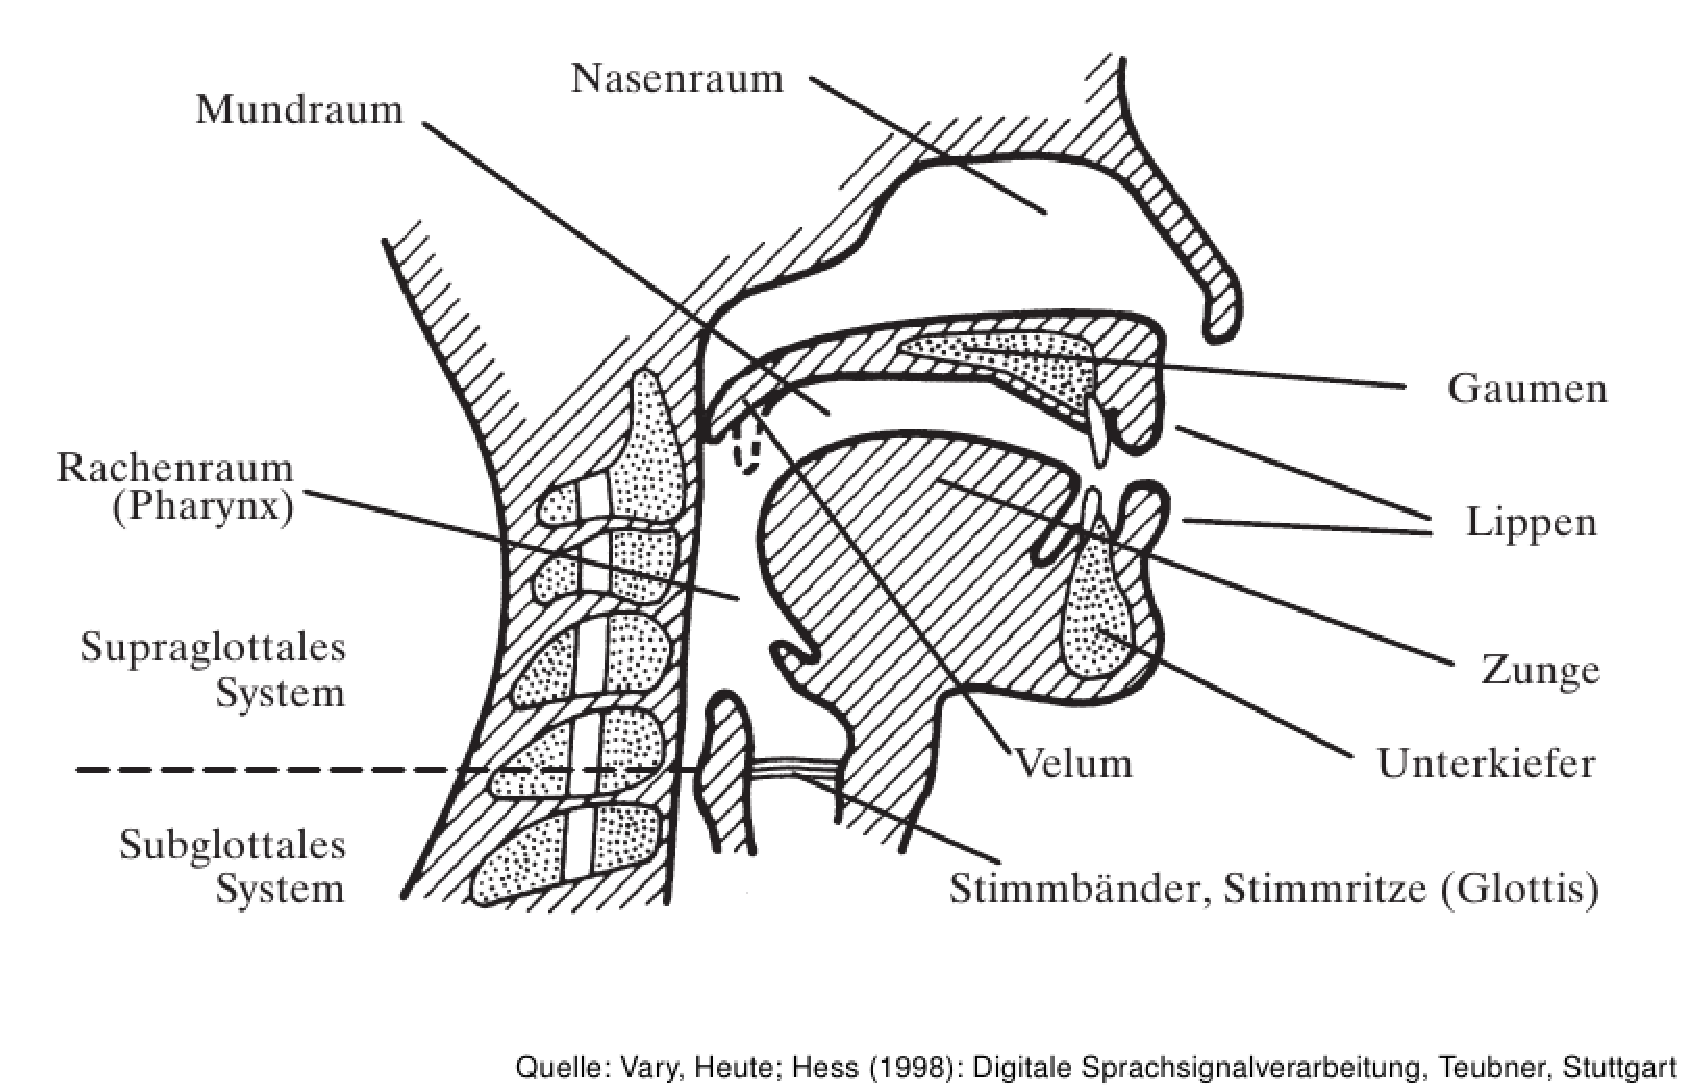
\includegraphics[width=0.7\textwidth]{Pictures/Chapter1_Lesson2/vokaltrakt-eps-converted-to.pdf}
    \caption{The vocal tract.}
\end{wrapfigure}

There are many speech sounds that we can produce and these sounds change for different languages. Probably the most obvious distinction that we can make between all of these vocal sounds is to separate them into voiced and unvoiced. Voiced speech sounds are those produced when our vocal chords vibrate. The best examples are the vowels.  These are sounds where the excitation signals are a periodic vibration of the vocal chords.  There are also unvoiced sounds. These are sounds where the glottus is not vibrating.  These are sounds such as the fricative  /sh/.  Plosives are also unvoiced speech sounds where there is a  complete constriction of the vocal tract and then a sudden opening such as /k/,/p/,/t/.  There are also sounds that are mixture of the two types of excitation such as /v/. \\
\\
Figure 2 shows how these different speech sounds look in the time domain. It was said that a voiced speech sound has a periodic excitation.  This can be seen in the periodic structure in the time domain plot.  The distance between two peaks in the plot is called the fundamental period, or the difference in time between the opening of the glottus. Fig 2b depicts an unvoiced speech signal.  Because there is no periodic excitation of the glottus, the excitation signal is more random in nature. This can be seen by the amount of zero crossings in the time domain plot.  Fig 2c shows a transition between two speech signals.\\

\begin{wrapfigure}{l}{0pt}
    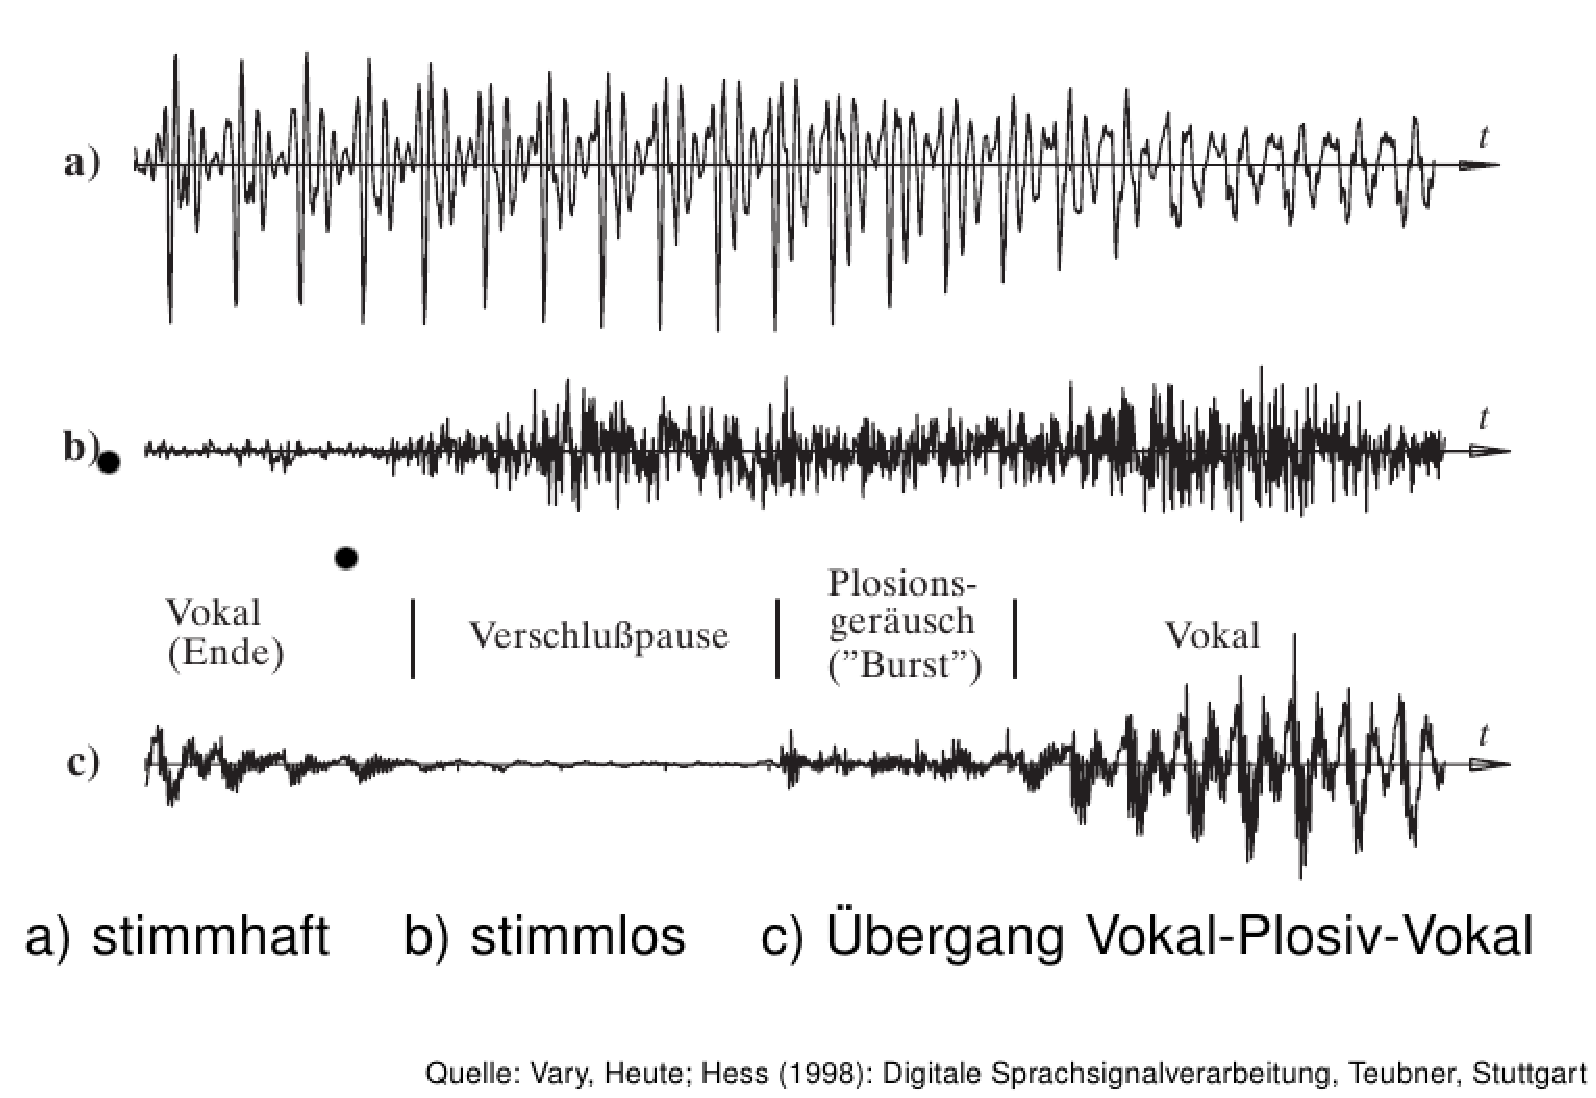
\includegraphics[width=0.7\textwidth]{Pictures/Chapter1_Lesson2/sprachlaute-eps-converted-to.pdf}
    \caption{Time domain signals of voiced and unvoiced speech.}
\end{wrapfigure}

Speech sounds convey meaning and because some of these sounds are different, however still convey the same meaning, there is a system to classify them. A phone is defined as the smallest speech segment with distinct physical or perceptual properties. To call a speech sound a phone is to say that there are no other segments of speech that are the same as that particular segment of speech.  Then there are phonemes.  These are the smallest segments of speech that can change the meaning of a word.  The phoneme consists of a set of phones, so phones are actually different realizations of a phoneme. All of the phones that belong to one phoneme are called allophones. One allophone is one phone of the many that constitute a phoneme. One phoneme can consist of many allophones.  For example, if you take the words ''kiss'' and ''kill'', they have very different meanings, however the difference is only in the phoneme at the end.  This is different with the words  ''cat'',''kit'', ''school'', ''skill''.  These all contain the phoneme /k/ but are pronounced differently due to the different vowel transitions and would, therefore, all be classified as different phones of the same phoneme /k/.\\
\\
Natural human languages have between 10 and 80 phonemes. These can be characterized by the way in which they are articulated, whether they are voiced or unvoiced, and in which place they are articulated.  Place of articulation is basically saying where the tongue is placed in order to produce the speech sound. The different parts of the vocal tract can be used to generate the different phonemes and are also differ across cultures.  The Americans use quite a bit of retroflex, rolling the tongue backwards to create a rolled  ''r' sound. Germans tend to use a glottal stop to distinguish between ''verreisen'' and ''vereisen''. There is a phonetic alphabet that can be used to describe all languages. Fig 3 shows this phonetic alphabet distinguished by place and type of articulation.\\

\begin{wrapfigure}{l}{0pt}
    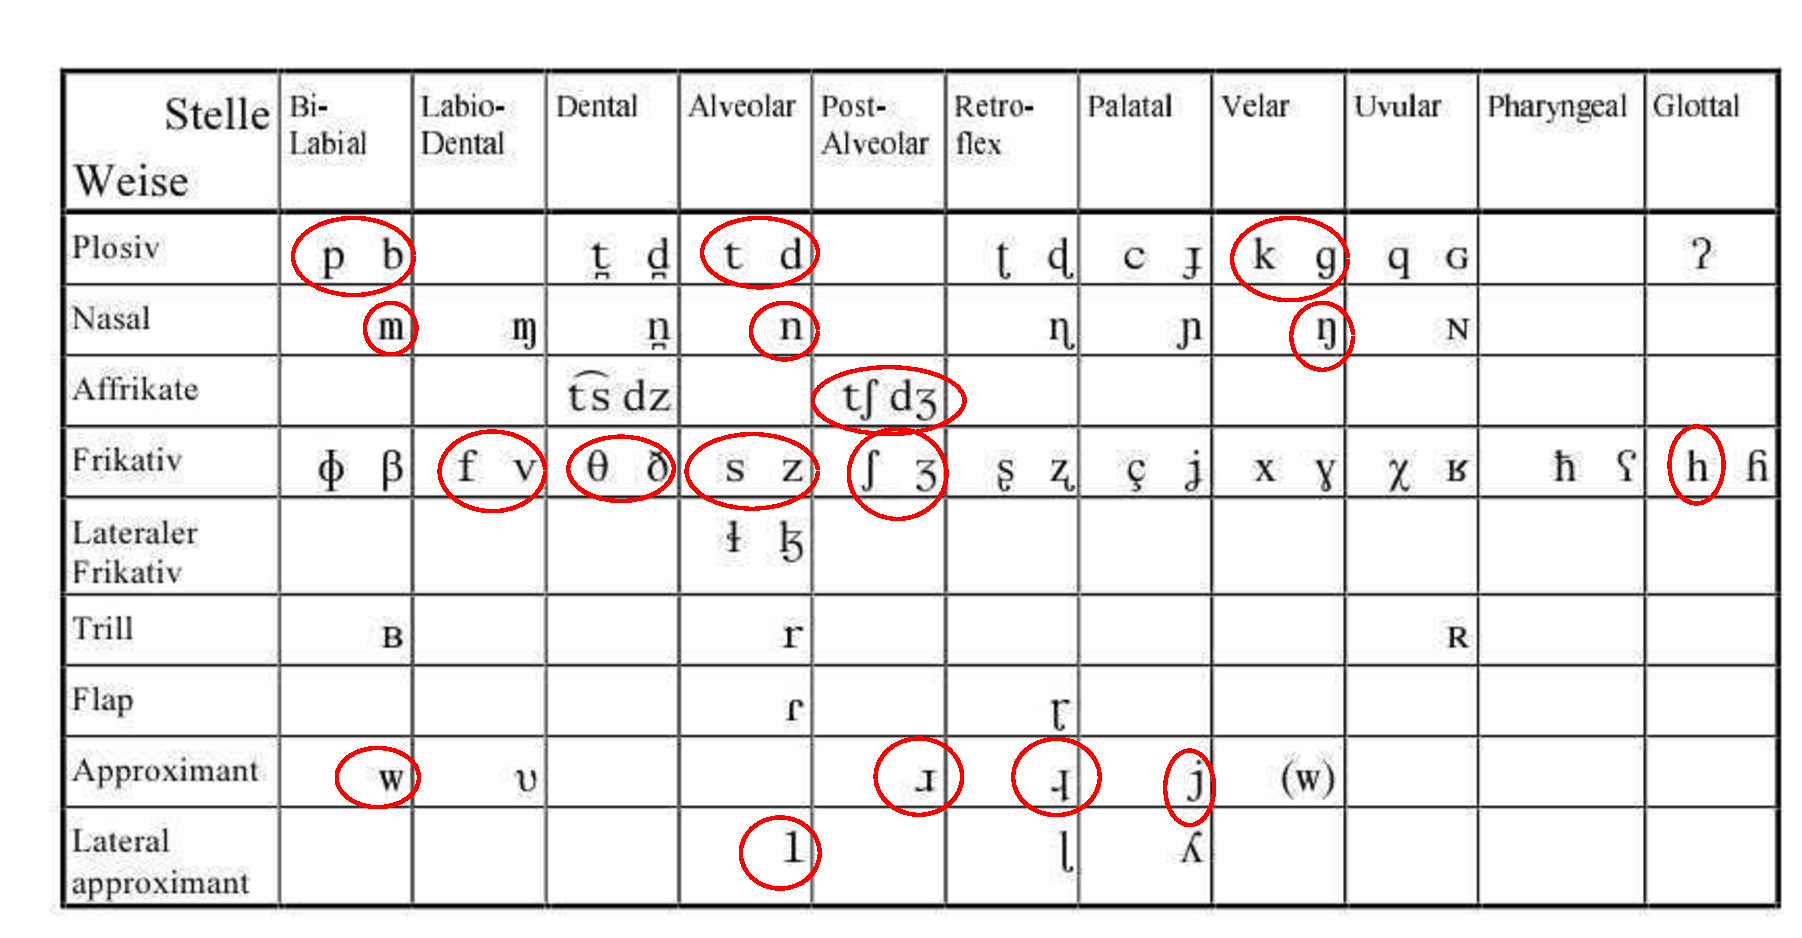
\includegraphics[width=0.7\textwidth]{Pictures/Chapter1_Lesson2/intPhonAlphabet_konsonanten_english2-eps-converted-to.pdf}
    \caption{The phonetic alphabet}
\end{wrapfigure}

Vowels can be distinguished by the position of the tongue in the oral cavity when they are generated.  These are called the cardinal vowels. As with the phonetic alphabet, we are looking for a language independent description. This is done by mapping the position of the tongue in two dimensions, Front to back and high to low, to the vowel sound.  This mapping can then be used to order the corresponding phonemes.  These are called the primary vowels as opposed to the secondary cardinal vowels which are less common and more difficult to say. On one axis, there is the positioning of the tongue from back to front, and then a different axis for the opening of the mouth. It is important to note that the secondary vowels are produced with open lips.\\

Co-articulation is a term used to describe the fact that we produce the same phonemes differently dependent on the content.  This is basically due to the fact that we cannot change our vocal tracts instantly, but there will always be a smooth transition of the tongue from one position to the next.  For instance when you say ''hen'',  it is usually an aveolar sound where the tongue is placed behind the front teeth. However if you say tenth, the /n/ is followed by a /th/, a more dental sound. Therefore, the /n/ will also be pronounced more dentally.  \\

Prosody is another important characteristic of speech.  It is defined as the rhythm, stress, and intonation of speech.  Mostly when people speak of prosody, they speak of the intonation of speech, the melody of the sentence that is said. However, the concept of prosody also encompasses the rhythm and the stress of a speech utterance. Prosody also carries information. It could be the difference between a question and a statement. If we ask a question, we usually raise the fundamental frequency at the end of the sentence.  We also use it to put emphasis on certain words. ''Put the GREEN ball on the table''.  ''Put the green BALL on the table''.  It also carries information about the emotional state of the speaker. For instance, if I yell, then this will usually have a different meaning than if I whisper.  


% CHAPTER 1 LESSON 3
\clearpage
\section{Source Filter Model}
\label{Source Filter Model}

The previous lesson introduced the method by which we produce speech. The lungs produce energy, in the form of airflow, that passes through the larynx where either oscillating vocal chords produce voiced speech or the airflow simply passes through to produce unvoiced speech.  This energy then passes through vocal tract, where the current positioning of the jaw, lips, tongue, etc. affect the shape and therefore the speech sound that is uttered.  This process can be modeled by a source filter model.  This assumes that we have a source, the airflow after it passes through the larynx, and then a filter which is defined by the resonance frequencies of the vocal tract. In this model, we assume that these two are independent. This is a very critical assumption and important to understand and would require, for example, that the resonances of the vocal tract are independent of the fundamental frequency of the excitation. The ultimate goal is to model this process mathematically and for this we have to understand what is really going on in the process. \\

\begin{wrapfigure}{l}{0pt}
    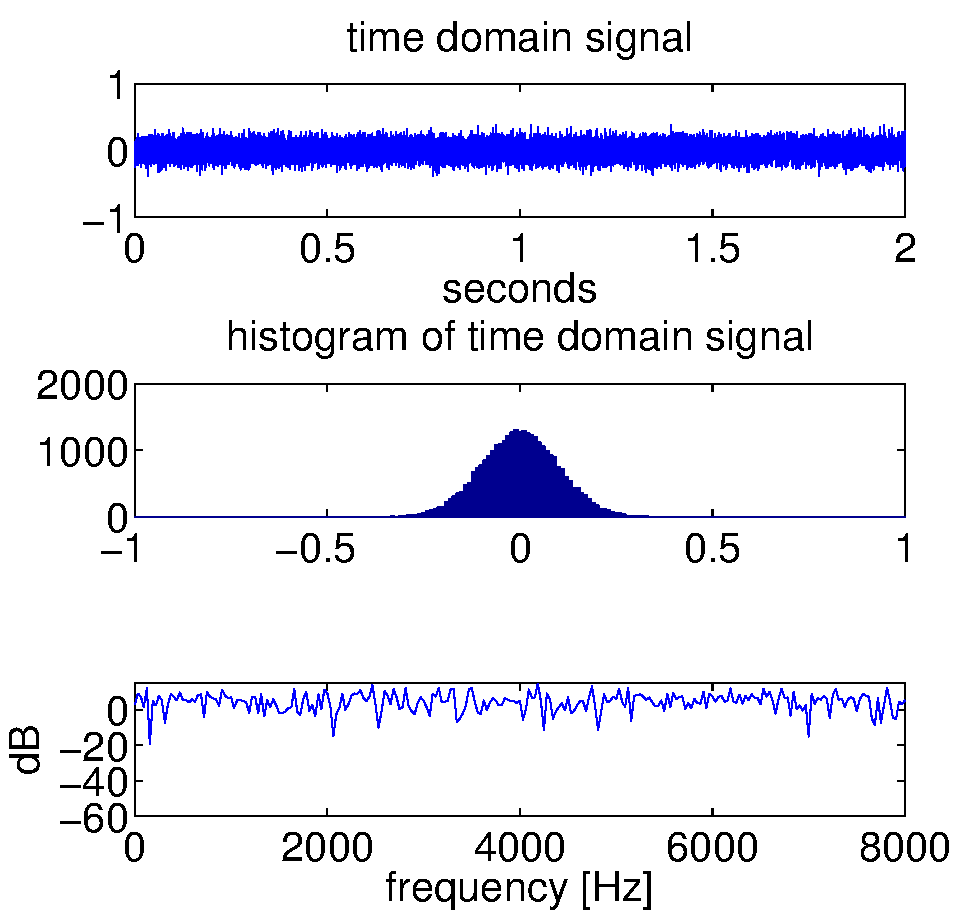
\includegraphics[width=0.5\textwidth]{Pictures/Chapter1_Lesson3/gaussianNoise-eps-converted-to.pdf}
    \caption{Statistics of white Gaussian noise.}
    \label{gaussNoise}
\end{wrapfigure}

The excitation signal for a unvoiced sounds is described  by turbulent airflow passing through the glottis. This can be modeled by using white Gaussian noise. The top of fig \ref{gaussNoise} depicts the time domain signal of white Gaussian noise. It is Gaussian noise, because a histogram of the samples in the signal will produce a Gaussian distribution. As can be seen in the histogram, there are more values close to zero than there are towards the edges. It is white noise, because a Fourier transform of the signal produces a flat spectrum.  The term ''white'' refers to a flat spectrum because in optics, white light as composed of an equal amount of energies of all frequencies, whereas light that has more energy in lower frequencies would be red.\\



For a voiced excitation, the vocal chords open and close periodically. If we look at the glottal flow behind the larynx, what is observed is a periodic form. First, we start with closed vocal chords, a closed glottis. Next, as we produce energy with our lungs, we push air and the glottis opens because there is an increased pressure that builds up at the base. As the glottis opens, the pressurized air can now escape and the thus, the airflow increases and by Bernoulli's principle, the pressure decreases. Because the vocal chords are under tension, this decrease in pressure allows them to snap shut to begin the process again. This is the mechanism behind voiced excitation. \\

\begin{wrapfigure}{l}{0pt}
    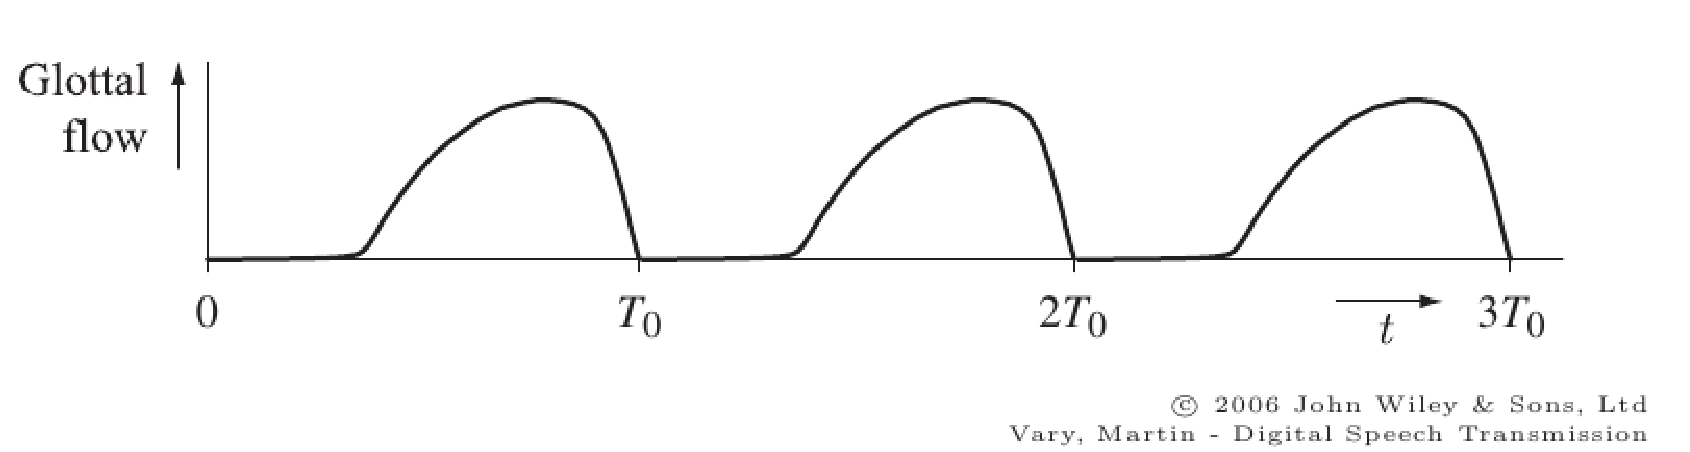
\includegraphics[width=0.5\textwidth]{Pictures/Chapter1_Lesson3/glottalFlow-eps-converted-to.pdf}
    \caption{Glottal flow over time}
    \label{glotFlow}
\end{wrapfigure}

 The two forms of excitation can now be described in a simple model. In the unvoiced case,  a noise generator can be used to produce the excitation energy.  For voiced speech, a pulse train in the time domain can be used with a peak to peak distance of the fundamental period, \begin{math}T_0\end{math} This will model the opening and closing of the glottis.  It is then necessary to have a switch that chooses between the two forms of excitation and some form of detector that can determine which excitation is present in the current speech signal.  There are also mixed excitation sounds, so one could also imagine there being a weighted summation of the two excitation signals, so we could have something that's a little more complicated like a weited summation to produce mixed excitation signals. \\

The next step is to model the vocal tract as a filter through which the excitation signal passes. The vocal tract can be thought of as a filter because it will have certain resonance frequencies similar to the resonances of a tube. In fact, the vocal tract can be simplified by using a tube model in which there is one input and two outputs, the lips and the nose. This can be seen in fig \ref{tubeModel}, where the tube on the bottom represents the oral cavity with another tube on top representing the nasal cavity.  The tubes will be separated by a switch that models the vallum.  Each tube will have its own resonance.  By modifying the shape of the tube, different resonances would be produced thus producing different speech sounds .\\

\begin{wrapfigure}{l}{0pt}
    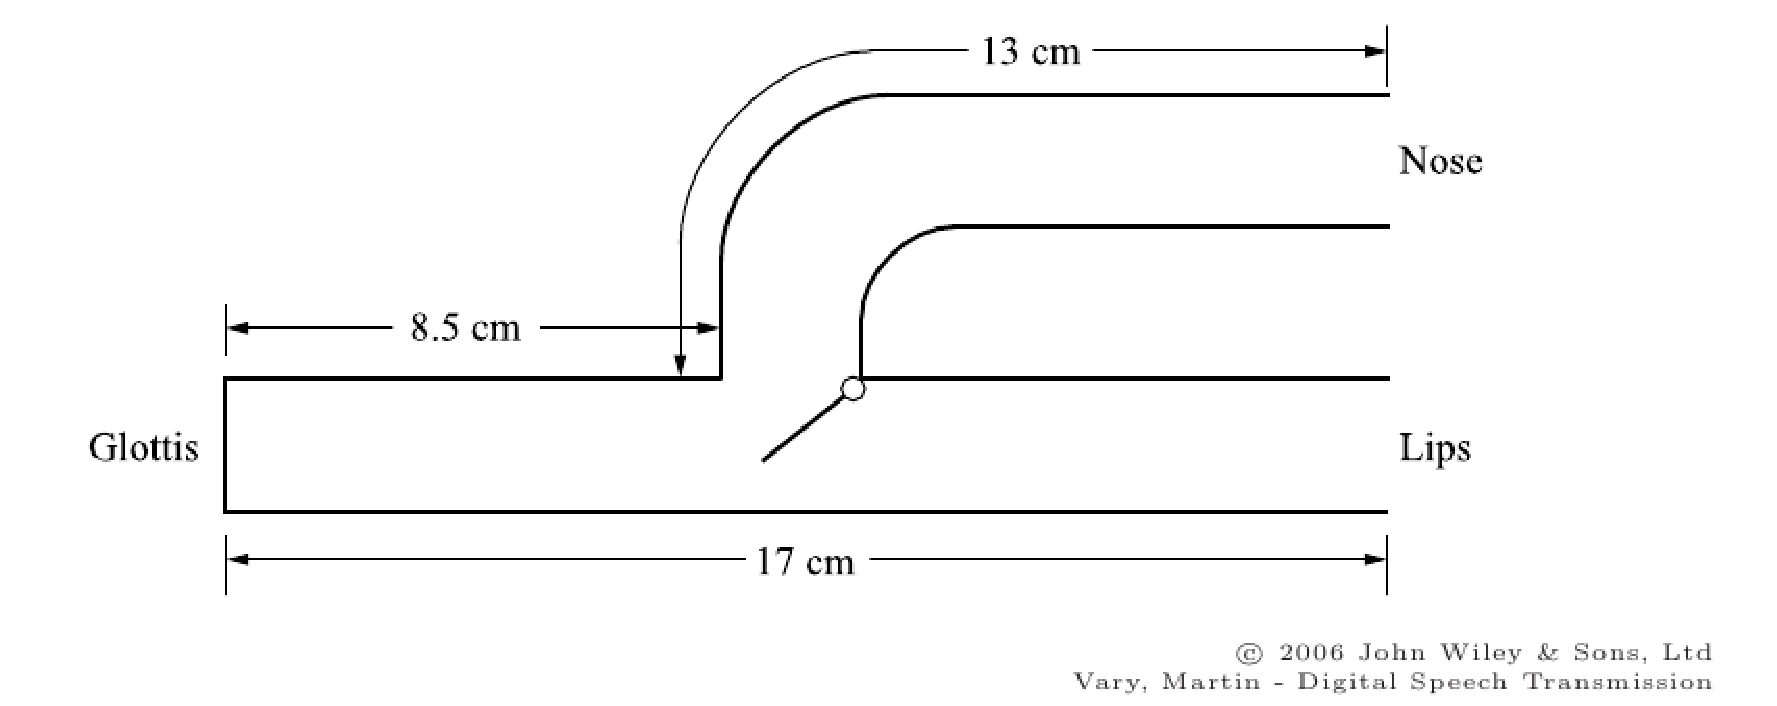
\includegraphics[width=0.7\textwidth]{Pictures/Chapter1_Lesson3/vocalTractSimple1-eps-converted-to.pdf}
    \caption{Simplified model of the vocal tract.}
    \label{tubeModel}
\end{wrapfigure}

From a signal processing view, the vocal tract filters the excitation signal to produce a speech sound. Mathematically speaking, this is represented by a convolution in the time domain and a multiplication in the frequency domain. The vocal tract can therefore be thought of as a transfer function. The spectrum of this transfer function would contain certain resonances. This can be seen in fig \ref{transFunc}. In signal processing, these are called formants, the resonances of the vocal tract. Formants contain important information because they decide what speech sound is being produced.  When the spectra of the excitation signal and the vocal tract transfer function are multiplied, what is seen is the result of what would happen if we did a frequency analysis of a recorded speech sound. The influence of the excitation signal and the vocal tract can both be seen in the final signal. It is very important to understand that these are two independent signals in our model. Notice that at the bottom of fig \ref{transFunc}, the formant peak is not seen. It lies between the two peaks of the harmonics because the final signal is an almost sampled version of the vocal tract function. Babies are very skilled at aligning the fundamental frequency with the formant, because this is when they scream the loudest! If the harmonics are between the peak of the formants, the energy in the final signal would be lower as opposed to the harmonic being aligned with the formant.  The peaks of the formants are given by the multiple peaks seen  in the transfer function, whereas the fundamental frequency is given by the first peak of the fine structure or the distance between two neighboring peaks.\\

\begin{wrapfigure}{l}{0pt}
    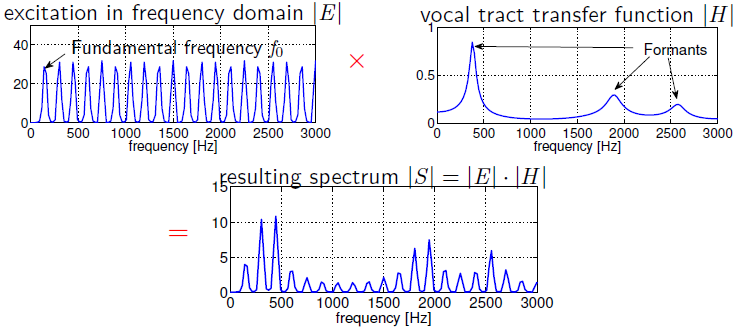
\includegraphics[width=0.7\textwidth]{Pictures/Chapter1_Lesson3/Transferfunc.png}
    \caption{Transfer function of the vocal tract.}
     \label{transFunc}
\end{wrapfigure}

Formant freq vs fundamental freq.  
Formants are imporatnt becasue they define the meaning of a speech sound.

We can then draw a formatn map with this information.  If we look at the map, we can see a caertain area  where phonemens have their formants. How lare the area is depends on the database used to create it .

It is imporant to understand the difference between fundamental frequecny and formants.  The formants carry the meaning where as the fundamental frequency refers to the excitiation signal and carries no real meaning (only with respect to tintonation prosody)

So for simple model of speech production there are certain parameters taht we need to know.  We would need to know: voiced/unvoiced speech signal to switch our excitiation and for this one, we would need to know our fundamental period, and our voacl tract transfer function.


% CHAPTER 1 LESSON 4
\clearpage
\section{Hearing}
\label{Hearing}

The ear, ruglhly speaking consists of different parts, the outer ear, the middle ear and the inner ear. the outer ear consistrs of the pinna the ear canal and the ear drum and the middle ear consist of the jkahsfda stapus which work like a leather.  The inner ear consists of the cochlea which is where we perceive sound and is where the auditory nerve is attached. Sound aves travel through the ear canal and cause the ear drum to vibrate and we have this lever here so we transistion from the large area to the samall area and here we would have then the travelling wave travelling through the cochlea. Here we would have the basilarmembrane.

The intersting thing is that the basilar membrane does the frequency to place transformation meaning that we have a travelling wave that will have its peak at certain point in space, for instance if we have a tone a 3500hz then it would have its maximum at a certain point if we have a high frequency tone the maximum would closer to the base of the badilar membrane so the point where the stapus, while if we have lower frequenceies , the resonances will be toward the apex.  so the tip of the cochlea and thats very imporatn becasue it means that we also perceive sound in the frequency domain m,eaning that humans perform a frequency analysis of the signal . Thats also why this frequency analysis that we use is so natural for us because it is also how we perceive sound .

If we look a little closer, at a cut through the cochlea we will see these tubes that wind up.  The interesting part is the basilar mnembrance and the ortgan of corti  where we have the hair cells.  What happens is that there will be a travelöling wave that will cause this part to move against the tectortial membrnce so that we will have the movemnet of the hair cells and they will then fire through the auditopry nerve and then the brain will have a percepotion of sound .

SO this is the auditory sensation area for a normal hearing person, so we have acertain threashlod of hearing here we see the frequecny axis on a logarithmic scaling. So we can see that at lower frequencies, we need more energy to perceive sound than at higher frequencies up to a caertain order.  Frequencies below 20Hz we are not able to perceive, at least not throught the cohclea and also at higher frequencies, we have problems as we get older. At the top is the level of pain. If we hear a sound at a level higher than the line for an extenden period of time, we will start to have hearing damage. We can see that speech fills a certain range in the auditory senstaion area.   Interestingly, the area where all the formants are is also the area where our ear is most sensitive. Quite conveninet It means that our ear is optimized for speech perception. (or the other way around) We see taht music has a wider range in frequency.  If you listen to the radio we hear that it sounds difffernt but we can still understand everything that is being said, this is because we still transmit the important formants even though the music range is much wider.

So what happens if we are hearing impaired or if we experience a sernsory neural hearing loss? So what happens approximately, or simply speaking is that the level of pain approx dont change, while the threshlod of hearing is increased.  We then need to amplify soft sounds but if we would just linearly amplify the level of sounds, we would o that beyond the level of pain and thats why we need compression algorithm in hearing aids, so tha twe amplify soft sounds more than loud sounds.  This decreases the SNR and therefore requires some noise reducxtion to enhance the signal to our hearing aid. 

Its interesting to note that there are different types of hearing losses.  The conductivbe hearing loss is the one can be traeated more easily that a senorsneural hearing loss  because it means that the sound is not properly conducted by the outer ear or the middle ear. The bomes could stiffen The sound is still perceiveable, but attentuatoed which also means that you can also treat it rather well with a hearing aid by amplyfying the sound. Sensorineural hearing loss is for instance what we have with th age related hearing loss so we get older then our hair cells die. They can also die because of trauma for instance if you are in very noisy or loud environment or if there is a gunshot. This can dmage the hair cells and then there is nothing that we could do at this time.  This sensory neural hearing loss is often accompanied by tinnitus where when one doesnt hear well, instead they hear a ringing. And then what else happens is that soft sounds are too soft and loud sounds are too loud which basically measn that we have this reduced area in the auditory sensation map. Whats also problematic is that the sensory neural hearing loss goes along with a decrease in frequency resolution meaning thta even if you do a audtitory test, you can still preform well to some extent, but still you have trouble when you want to perceive speech in noise cause the frequency resolution of your auditory perception is decreased. And this means that we cannot so well distinguish between speech commands. And that means that we have a decreased speech understanding in noise and for this reason again noise reduction is a more important aspect.

Current hearing aids commonly implement multi microphones. In this model there are three different microphones that are channeled to an analysis filter bank where a time frequency analysis is performed similar to what we do in the cochlea. Then we we do a directional processing with the microphone. Because there are multiple microphones, we are able to cancel out the sounds that come from a specific direction while keeping the sounds that come from the fron for instance unattentuated. This is also done in hearing aids. Basically you can choose whom you want to listen to by lookingat that person. However this is not a very narrow beam, but a very broad beam.We can make this beam more narrow, we could have, for instance a binaural hearing aid where we have two hearing aids that communicates meaning that we have microphones placed further apart because these microphones are only on one hearing aid so if we pull them apart, we can produce a more narrow beam and this is  well technology that is evolving, but we must transmit this information to the other hearing aid.  This can be done with a wire, or wirelessly, but then we have a large energy consumption.  But in the simplest case, we transmit control information, for instance volume control makes more sense if both hearing aids are in the same state. The same holds for calssificaton of the background noise.  Many hearing aids have auditory scene analysers where they for instance let say if you are in a noisy environment and we want to do speech communication then you want to turn on the noise reduction in order to perceive speech better.  But if you are at a concert, you listen to some music then you dont want noise reduction depending on your tastes i music. :) SO that would mean that the hearing aids would have certain algorithms that control certain parameters of the auditory processing. There is also then a feedback cancellation stage where we cancel out feedback loops. 




% CHAPTER 2
\setcounter{chapter}{1}
\chapter{Pitch}
\thispagestyle{plain}


%Box with Learning objectives should be at the beginning of each chapter

\begin{corollary}

	\hspace*{10mm}
	
	\vspace{5mm} %for optical corrections
	% optionaler Text	
	
	\begin{itemize}
			\item Fundamental Frequency Estimation

	\end{itemize}
\end{corollary}

\newpage

%Einf�hrung in das Kapitel



% CHAPTER 2 LESSON 1
\clearpage
\section{Fundamental Frequency Estimation}
\label{Fundamental Frequency Estimation}



%Einf�hrung in das Kapitel

In the first part of this lectrure, we talked about very general things such as how speech is produced through the source filter model, the midel on how we produce speech.  The question now is if we have a speech signal, how we do we get the paramters out of it? So we said for the excitiation signal, we said that the parameters are voiced or unvoiced, and if its voiced, what is the fundamental frequecncy. So this again is an example of unvoiced and voiced sounds, and as we can see, the unvoiced sound is rather noise like, doesnt contain periodic structure, whereas the voiced signal has a periodic structure and the goal now is to estimate the fundamental frequency or the fundamental period which are reciprocals of each other. 

This is a plot in the short time fourier transform domain, so we have here the time axis and here the frequency axis, with the color being the enegery of the signal, with read being lots of energy and blue being less energy. And then we see here the fundamental frequency and its harmonics.  We can see that at the fundamental frequency, we have energy in the signal. Also we see that the distance between the line are the same, becasue the distance between two harmonics is the fundamental frequency. 

So what I'm trying to say is that it can be that fundamental frequency is very much attentuated by the filter function of the vocal tract, but the excitiation signal will still be there. The fundamental frequency, fo is an important paramter in speech signal processing.  We need it in many algorithms, for insatnce speech coding, also in speech synthesis, for instance if you have this voder you have to controil this pedal, meaning that we have to move the fundamental frequency. In coding it is also similar, you can use such a parametric form of speech production for a speech coder and then the fundamental frequency would be one paramter that we have to ttransm,it to a receiver site. also for speech enhancement, thje fundamental frequency can be used for instzance if our signal is filklerd with noise, what you know ....
so assume there is whit noise filling up the gaps of a spectrogram you could attenutate the noise where speech is not present If you know the fundamental frequency you can keep those bits where the fundamental frequency is and reduce the enegy in the bins where the spectrum is noisy.  And with this, you can do speech enhancement. There are much more enhanced techniques, but this is just to give you an idea.  

Very often in speech processing, we use the word pitch synonymously with fundamental frequency, but it important to realize that pitch is a perceptual quality, where pitch is a perceived quality of a tone, whereas fundamental frequency is a physical parameter. And what is the difference. If you ask people how they perceive the pitch of a tone this is also influenced by the loudness. So something would have a different pitch perception if its louder o softer. 

The range of the fundamental frequency is between 40 and 600 Hz although 600 Hz is a bit on the high side.  This is something that would only be seen in children and typical speech fundfamentla frequencies are around 100Hz for male speaker, and about 200Hz for female speakers . This is just a rule of thumb
.

This is the residual effect. This is again just to give you an idea of what we mean when we talk about fundamental frequency. The idea is that we perceive the fundamental frequency of the sound even when this fundamental frequency is not part of the signal.  So what I am saying is if you in the frequency domain have a spectrum like this and then we apply a lowpass filter, we would still perceive a fundamental frequency and this is the case in telephone speech. In telephone speech, due to very historic reasons the low frequencie are not transmitted so basically only frequencies above 300Hz are being transmitted and as we learned before, the fundamental frequency is usually below this and so is not trransmitted.  But still, we are  distinguish netween the male and the female speaker and we can realize who is calling us and so forth becasue what we use to get an idea of the fundamental frwuency is the distance between harmonics. In fact, if we play a tone at 200HZ and a tone at 300Hz and we sum them up and play ithem together the resulting tone sounds lower because we are perceiveing the fundamental frequency. If we look at the signals below figure . If we sume both tones and look at the time domain signal, we'll see that the distance between the peaks is 100Hz. If we do a DFT of the signal, we'll see no energy at 100Hz because all we did was perform a linear addition of the two tones, and because of this, there acnnot be any new frequency coming into the signal.  However the fundamnetla period is till 100Hz and we perceive a lower tone. And so we can even still in telephone speech, distinguish male and female speakers. 

There are still some problems when we throw away this high frequency information especially with speech sounds containing more high frequency information such as plosives.  It is almost impossible to distinguish some phonemes such as s and p in telephone speech when played by themselves. However, when heard in context they are still intelligible.  This is also seen when we must spell things over the phone and use a spelling alphabet such as c like charlie. In the telephone speech that we have today, we throw away a lot of information but people dont complain about it much becasue they are used to it. It is more expensive to transmit more data. There is also a problem with compatiblility.  If you have a phone the transmits wide band speech but the other person does not, we would not use it as much. FOr instance, VoIP there are softwares that use wide band speech codecs.  We hear more natural speech sounds. 

How do we estimate it? The easiest way would be to take a time doimain signal and for instance and measure the time between the zero crossings. We could also measure the distance between the peaks.  What we also see here is that often, we dont have perfect periuodicity so this period does not look exactly like this one, but it looks similar. And you can also imagine that there is noise in the signal making it much more difficult to find these points where the periodic structure repeats. In other words, you can so this but it is prone to errors. But as said before, this is difficlut to do in an automatic setting, if we wanted to have a machine where we just have a recording from a microphone that stands somewhere in the room or it might be a microphone in the cell phone and youre tryong to estimate the fundamnetal frequency it is very difficult to do it based on this concept. The better way to do it is to use the autocorrelation function.

The autocorrelation fucntion is given as the expected value the signal x(n) and the shifted version of itself.  If x would be a complex valued signal, then it would be the complex conjugate of the signal. But for time domain speech signals, this is not the case. So we can forget about the asterisk there. But what we see is that you take the siginal and shift it by lambda, multiply it and then take the expected value.  The expected value is then defeined as the integral over these two signals multiplied by the joint probability density function of the two signals. This is the formal definition. In practice you cannot really knoe this expected value because you don't really have the joint probability density function, so what we have to do is estimate it by replacing the integral with a summation over realizations of your signal. So what you do is mulktply the signal by itslef shifted by lambda and then average over a certain segement ie 30ms. And this we do for different lambdas, different shifts of the signal against itself and this will be a measure of the self similarity of the signal. Why is this? Lets say you have a periodic signal in time domain and now you shift it by zero, ie you dont shift it, you would have the same signal. So now we multiply the two signals and that basically means that, where we have postive values in one signal, we will have positive values in the other meaning thatthe product of the two is positive, and if both are negative, then the result will be positive.  And then we sum up these signals we'll get a large value.  On the other hand if you shift it by a differnt factor, lets say like this we can imagine that the result will be smaller because there will be parts where the one signal is postive and the other is negative and vice versa so meaning that if you do the multiplecation and sum it up over time, then you'll get definitely a smaller value tahn if you do this without .....So it will begin high and then decrease, but then achieve another maximum at the period.  

It is also important to note that the Fourier transform of the autocorrelation function is called the power spectral density.  It is also interesting to look at the power spectral density of a signal and not only the autocorrelation. To understand this concept, for white noise what we would have, per definition, a white noise signal means that succesive samples of a signal are uncorrelated and that means that for the autocorrelation function we would have a peak only at zero where it is the same, but for any other shift of the signal, you would have that the autocorrelation cancels out and goes to zero. This is what you observe here so this is a measured autocorrelation function so here we didnt take the expected value but replaced it with an averaging over n samples and then what you see is that you have some some noise left so it doesnt really goto zero. But this is just an artifact of the measurement. Ideally speaking it would goto zero if you would have the real statistical expectation. If you look at the Fourier trandform of this, you know that the FOurier trandform of a delta peak corresponds to a flat spectrum. So what we would expect is a flat spectrum, but what you get is something noisy. So this is flat in the mean but noisy. But the main thing, then important thing to realize is that the white signal has a flat and thus white spectrum.

So how is this for  speech? For speech, successive samples are not uncorrelated but they are correalted so especially for voice, what you would observe is that you would get a peak at lag zero, but also peaks at multiples of the fundamental period and now, what you would do for fundamental frequency estimation, this is also something that you would do in the computer excercise is to take a speech signal of frame Lenght N lets say 30ms, compute ACF, so shioft the signal against itself and then you need to find the first peak because this is what corresponds to the first period. SO the easiest way to do this is to do a maximum search.......

If you look at the spectrum of a voiced speech sound, it looks like this.  What we see here is the fundamental frequency and multiples of it being the spectral harmonics and what you would also see is that there is a spectral envelopewhich is due to the resonances in the vocal tract. .

WHen you do this excercise and compute the ACF, you need to deceide on a certain window length, the number of samples N that you choose. There is a certain tradeoff. If you have a window length that is just as large as one period or shorter, then the algorithm will not work very well becasue you cannot really shift it by one period and this also shown in this plot of the estimation error for the fundamental period .So if you take your window to shoret, you get bad performance, on the other hand,m if you take your window length longer hat means you would have multiple periods within this window that makes the estimation of the fundamental frequency more robust but of course there is a limit becasue the fundamnetla frequency will change over time. If we wouold speak at a constant fundamental frequency all of the we  time, then of course we would sound robotic. 30ms is roughly the range wher threee periods of the fundamental period fit into one window at a fundamnetla frequency of 100Hz so you would have roughly three periods for male speakers. 

There are also variants of this method, so many pitch estimators are based on the Autocorrelation function. But there are alos alternatives.  A famous model is called YIN and its based oon the difference function.  The idea here is that you take a signal and the same signal shifted by a certain valueand subtract the two. if tois exacltly the fundamental period and the signal is perfectly periodic then this difference will goto 0. Its like having a sinusoid and then shiofting the sinusoid by one period and then subtract the tow then the difference will be zero because the signal is exaclty the same by its fundamnetla period. And so this idea can also be used to design a fundamnetla frequency estimator. So the idea is that you take the square of this difference function and then average over N samples.  And then you get a value D and this algorithm would try to find the to that minimizes ths D.  This method is very much related to the autocorrelation function because you see that the summation looks very similar to the autocorrelation defintion. SO what we can now do is solve this thing you multiply out this square, and then what you see is that this d function actually consists of the autocorrelation function at time  x(t) at t + To - the estimate at time t with lag to.

And interetstingly if you have a perfectly periodic signal, you can show that the autocorrelation function at time 0 and the autocorrelation function at time t+To you would get exaclty the same result. In that tcase, the two methods are identical, however in practice, this is not the case, so we can make measurements of the error and we can see that ACF has a larger error than this difference function method. This is a trick used in this YIN approach.  There are also more tricks used to reduce the error even further.  




























As introduced in the previous sections, speech can be modelled as being produced by two types of excitiation. Unvoiced speech is rather noise- like, lacking a periodic structure.  It is created from air flow being blown through the vocal tract by the lungs. The position of the vocal tract gives a spectral shape to this turbulent air flow.  Voiced speech is generated by the glottus opening and closing, thus regulating this air flow in a periodic manner.  The period of this opening and closing is referred to as the speech fundamental period, the inverse of which is the fundamental frequency.

Speech fundamental frequency is often synonymously used with the term pitch.  It is important to note,however, that speech fundamental frequency is a quantitative value that is associated with the opening and closing of the glottus, whereas pitch is more qualitative, influenced by the loudness, length, as well as frequency of the speech.

Because fundamental frequency has this effect upon our perception of speech, it becomes an important parameter in speech signal processing and has important implications in speech coding, enhancement, modeling, and recognition.  It is therefore necessary to develop tools in which this parameter can be estimated.  For this, the advantages and disadvantages of several methods are explored.



	It is first important to note that fundamental frequency can still be estimated from its harmonics, even when it is not, itself, present in the signal.  This is exemplified by telephone speech which is generally band-pass filtered between 300Hz and 3400Hz in order to minimize bandwidth per user.  This range preserves the formants necessary for speech comprehension, however does not include the fundamental frequency.  
	
	How the fundamental frequency is still preserved is obvious when we look at the superpostion of two harmonics of a fundamental frequency.  If a signal has a fundamental frequency of 100Hz, there will be harmonics at 200Hz,300Hz, etc.  If this signal is high-pass filtered at 150Hz, the perceived signal will be a superpostion of the harmonics above 200Hz.  As can be seen in the accompanying figure, the sum of a 200Hz tone and 300Hz still displays a fundamental period of \begin{math}\frac{1}{100Hz}\end{math}, however the 100Hz tone is still not present in the frequency spectrum.

\vspace{-5mm} %for optical corrections


\subsection {Fundamental Freq Estimation by zero-crossing and peak measurement}  Prone to errors and hard to automize in an algorithm.  



\subsection {Fundamental Freq Estimation by autocorrelation fucntion}.  

We now define the autocorrelatiion function as:

\begin{equation}\varphi_{xx}(\lambda) = E(x(n)x^*(n + \lambda) = \int^{\infty}_{-\infty} \int^{\infty}_{-\infty}
uv\end{equation}
% p^{x(n)x^*(n + \lamda)(u,v)du dv} \end{equation}


A signal is white if succesive smaples of the signal are uncorrelated.  This implies that it has a flat power spectral density and has only one peak at lag zero.

For speech, succesive samples are correlated therefore we will see peaks at lag zero and multiples of the fundamental period.  

Window length must be longer than the fundamental period, but not so long that it cannot account for changes in the fundamnetal frequency. 







% Chapter 3

\setcounter{chapter}{2}
\chapter{Spectral Trandformation}
\thispagestyle{plain}

%Box with Learning objectives should be at the beginning of each chapter
\begin{corollary}

	\hspace*{10mm}
	
	\vspace{5mm} %for optical corrections
	% optionaler Text	
	
	\begin{itemize}
		
			\item Fourier transformation (continuous time vs. discrete time)
			\item Digitization of speech signals (time-amplitude)
			\item Discrete Fourier Transform (DFT)
			
	\end{itemize}
\end{corollary}
\newpage

% CHAPTER 3 LESSON 1
\clearpage
\section{Fourier transformation (continuous time vs. discrete time)}
\label{Fourier transformation (continuous time vs. discrete time)}


%Einf�hrung in das Kapitel

Usually in signal processing, what we would like to do is modify a signal to some extent. For this it is important that the properties we want to modify are easily accessible. In the previous chapeter, we already saw that the fundamental period is an example of a speech property that is not so easily accesible in the time domain. It can be seen in the time domain, however it was shown that time domain based algorithms (ie.peak and zero crossing measurement) are prone to errors. It can then be beneficial to look at some transformation of the signal. Using the example of fundamental frequency estimation, it was shown that the autocorrelation function makes the estimation of the fundamental period more robust. A different concept is to look at the frequency content of signals. For instance, we have already seen some spectrograms of voiced speech. These produce a time/frequency based visualization that allows us to see the fluctuation of the spectral envelope.  It was shown that the spectral envelope is formed by the vocal tract and corresponds to the meaning of a sound and is what we use to distinguish between two phonemes. A narrow-band spectrogram can also reveal the fundamental frequency and its harmonics.  \\

This process of decomposing a signal into its frequency contents in order to make certain signal properties more accesible is known as Fourier theory. In Fourier analysis a signal is basically correlated with complex exponential functions, and because any exponential function can be written as a sum of cosine and sine functions, this means that it is correlated with cosine and sine functions. Because these exponentials can be shown to be linearly independent of each other(eigenfunctions), Fourier anaylsis preserves all of the original information and is therefore a completetly invertible function. This implies that no information is added or removed in the analysis and that it is simply a different way of representing the signal.  Certain attributes of the signal are made more visible whereas others are not visible any more. \\

 A pure tone is a tone that consists of only one sinusoid with a certain amplitude, frequency and phase. Note that this also includes a cosine function as a cosine is just a sine with a 90° phase shift. This pure tone is what we call a sinusoidal signal, and one of the key concepts of Fourier theory is that any periodic signal can always be represented as a sum of weighted sinusoids at the signals fundamental frequency and its harmonics, integer ultiples of the fundamental frequency. This is known as a Fourier series analysis.  Fourier theory can also be extended for arbitrary (non periodic) signals. The signal can then be shown to be composed of the integral over all frequencies that are in the signal, the spectrum of the signal.  This process is known as a Fourier analysis. \\

Figure 3.1 shows an example of a fourier series analysis of a rectangular function. The top sinusoid depicts the contribution of the fundamental period to the analysis. The second signal is the sum of the fundamental and a weighted third harmonic. It can be seen that the sum is a bit more close to the rectangular function, and as the number of harmonics is increased, a better approximation to original signal is achieved. The figure on the right shows how to weight the harmonics to get as close as possible to the square wave, and it can be seen that the majority of the energy is in the fundamental frequency with an exponential decay for the higher harmonics.  Another way of thinking about it is that at the edges of the rectangular function, there is a very sudden jump in the time domain, corresponding to a very high frequency content. Theoretically, one would need infinitely many harmonics to model the signal perfectly.\\

\begin{wrapfigure}{r}{0pt}
    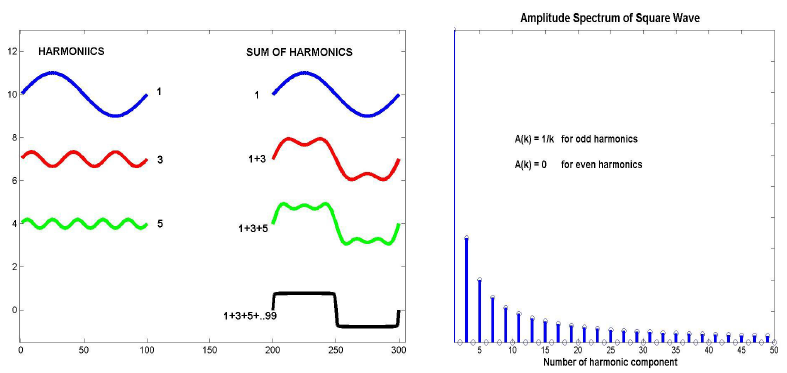
\includegraphics[width=0.7\textwidth]{Pictures/Chapter3_Lesson_1/FourierSquare.png}
    \caption{Fourier series analysis of a square wave.}
\end{wrapfigure}

Equation 3.1 is the mathematical representation of this process. The value, \begin{math}\cosCoef_0\end{math}, is called the DC offset and is the mean value about which the signal oscillates, in this case it is zero. The signal is therefore represented by this DC offset, and weigted contributions of sine and cosine functions at multiples of the fundamental frequency of the original signal. These weights are determined by correlating the original signal with cosine functions to determine the coefficients  \begin{math}\cosCoef_h\end{math} and sine functions to determine the coefficients \begin{math}\sinCoef_h\end{math}. Because the cosine function is an even function, whereas the rectangular function is odd, there will be zero correlation between the two. Therefore, the \begin{math}\cosCoef_h\end{math} coeffficients will all goto zero, leaving only the \begin{math}\sinCoef_h\end{math} coefficients to represent the signal. This can be seen in the right of Figure 1 along with the exponential decay of the weighting of the higher harmonics. \\

   \begin{tikzpicture}
\node [mybox] (box){%
    \begin{minipage}{0.50\textwidth}
    \begin{center}
    \begin{equation}x(t) = \frac{\cosCoef_0}{2}+\sum^{\infty}_{h=1}(\cosCoef_h\cos(2\pi hf_0t))+(\sinCoef_h\sin(2\pi 		hf_0t))
    \end{equation}
    \end{center}
  \end{minipage}
};
\node[fancytitle, right=10pt] at (box.north west) { Fourier series analysis};
\end{tikzpicture}%
  


Another reason why frequency analysis is a tool so often used in audio processing is that we also perceive sound in the frequency domain. This was introduced in the section on hearing regarding the frequency decomposition performed in the inner ear at different positions along the cochlea. This place coding implies that the cochlea performs a mechanical frequency analysis and that humans, in a sense, perceive sound in the frequency domain. This is the reason that it is quite natural for us to look at audio signals in the frequency domain. Computation can also be made much simpler in the spectral domain as convolution in the time domain corresponds to multiplcation in the frequency domain. This is often much easier to compute and is also another reason why spectral analysis can be the right tool to analyze certain signals.\\
  
  
  
%  
%  This is an example to get an idea of what frequency means what you can do is take a speech signal and filter out certain frequencioes andthen you get an idea of there certain contribuitions. SO this for instance is a speech signal with an audio bandwidth od 4khz. So if you throw away the frequencies higher than 2 khz we can stil understand but it doesnt sound nice anymore.  If we just look at the high frequency part, we only herar very little and it rather difficult to undertand and this is also because important formans are missing nowAnd if we just cut out frequencies between 500 and 1500Hz you can also get some odd distortions as opposed to the original.

  \begin{tikzpicture}
\node [mybox] (box){%
    \begin{minipage}{0.50\textwidth}
    \begin{center}
    \begin{equation*}
    X(\jmath\omega) = \int_{-\infty}^\infty x(t)e^{-\jmath \omega t} \mathrm{d}t
    \quad\quad\quad\quad x(t) = \frac{1}{2\pi} \int_{-\infty}^\infty X(\jmath \omega) e^{\jmath \omega t} \mathrm{d} \omega
    \end{equation*}
    \end{center}
  \end{minipage}
};
\node[fancytitle, right=10pt] at (box.north west) {Continuous-time Fourier transform};
\end{tikzpicture}%
   
    
  However, not all signals are periodic and eligible for Fourier series analysis.  In these cases, the continuous-time Fourier transform (Eq 3.2) can be used to represent any arbitrary signal. Any continuous time domain signal can be represented by a continuous frequency domain signal by bascially correlating the signal with complex exponentials over all frequencies, \begin{math}\omega\end{math}. And because complex exponentials can be represented with sines and cosines, this is like correlating the signal with sine and cosine functions over all frequencies, \begin{math}\omega\end{math}. In this sense, it is somewhat similar to the computation of the Fourier series coefficients, however the difference is that we now correlate over an infinite number of frequencies, not just the fundamental frequency and its harmonics.\\
  
   \begin{tikzpicture}
\node [mybox] (box){%
    \begin{minipage}{0.50\textwidth}
    \begin{center}
    \begin{equation*}
     X(e^{\jmath\omega}) = \sum_{\timei =-\infty}^\infty x(\timei ) e^{-\jmath \timei \omega}
      \quad\quad\quad\quad
      x(n) = \frac{1}{2\pi} \int_{-\pi}^\pi X(e^{\jmath\omega}) e^{\jmath\timei\omega}\mathrm{d} \omega
    \end{equation*}
    \end{center}
  \end{minipage}
};
\node[fancytitle, right=10pt] at (box.north west) {Discrete-time Fourier transform};
\end{tikzpicture}%
  
   
  
 The signals that we will be dealing with in digital speech processing will not be continuous, but discretized and sampled in the time domain.Therefore, we define the discrete time Fourier transform, DTFT. This is a transform with a discrete time index, \begin{math}\timei\end{math} but still a continuous frequency representation, \begin{math}\omega\end{math}. Here again,\begin{math}\omega\end{math} can take on an infinite number of values between 0 and \begin{math}2\pi\end{math}, wheras \begin{math}x(\timei)\end{math} is a finite,discrete representation of the original continuous signal. \\
  
    There are certain properties of the DTFT that can be related to the continuous time Fourier transform.  Looking at the definition of the DTFT in Eq2, we begin with the discrete time domain signal, \begin{math}x(\timei)\end{math}. To compute the frequency representation, instead of an integral, there is a summation.  The discrete time domain signal, \begin{math}x(\timei)\end{math} is  multiplied by phase shifted complex exponential functions and then summed. It is also important to note that, for the DTFT,  \begin{math}\timei\end{math} can only take on integer values. To return to the time domain, you would integrate over all frequencies again multiplied with these complex exponentials (conjugate?). Again these two transforrms are perfectly invertible meaning that there is no information lost upon conversion from time to frequency domain and vice versa.\\
    
 Because an integral and a summation are linear operators, the Fourier transform is itself linear. If you have a signal corresponding to the linear superpostion of two other signals, possibly even weighted with some scalar, then the Fourier transform of the sum of the two signals is equivalent to the sum of the Fourier transform of each signal. This is the basic defintiion of linearity and how we define a linear system. \\
  
 Very often in digital speech processing, we look at real valued signals in the time domain.  For example, a recording of an audio signal is real valued, implying that the spectrum is complex conjugate symmetric. This means that the real part is even while the imaginary part is odd. We can therefore also look at the even and the odd parts of the time domain signal separately. As introduced before, if  an even signal is correlated with a complex exponential, it is correalted with an even function, a cosine, and an odd function, a sine. The correlation between an even function and an odd will goto zero because of their opposing symmetries. When multiplied by the sine function, all values to the right of the origin will have equal, but opposing values, to the left of the origin, and the sum of the two will goto zero. \\
 
% So this means that the odd part of signal corresponds to the imaginary part of a spectrum.
% 
% Then a very basic property ist that the convolution, this is something you should all know.  A convolution in the time domain corresponds to a multiplecation in the frequency domain.
 
% Then a time shift, if you shift your signal in time, it corresponds to a taking the spectrum of a signal and modulating it with a omeag times the time shift.   It also goes the other way around if you shift your signal in the frequenccy domain, you have to modulate you signal in time domain. All of this properties are quite simple to derive.  All you have to do is the definitions of the FOurier transform and plug them in on one of the sides, and then you can derive all of these relations quite easy.  The last one is Parsevals theorem which also says the energy in a signal will be preserved when you take the Fourier analysis of a signal.


    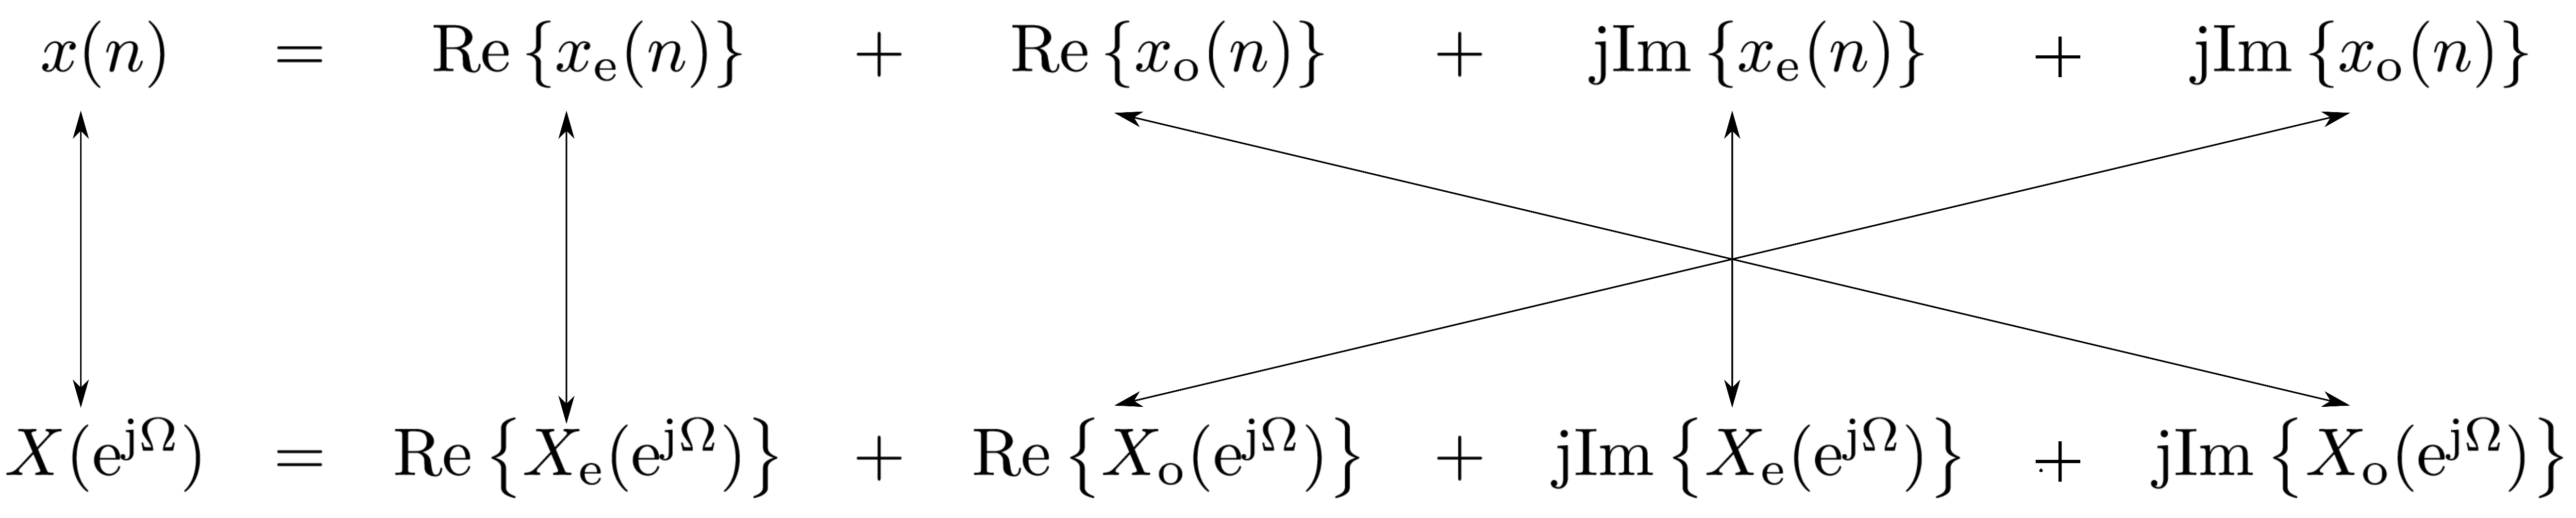
\includegraphics[width=0.7\textwidth]{Pictures/Chapter3_Lesson_1/dftSymmetry2-eps-converted-to.pdf}
   
 
 So, symmetry relations.  So this again relates to the analysis of the even and the odd part that I talked about before.  SO of coure, you can take a signal and it Fourier transform and you get the complex valued signal in the spectral domain . As we said, if you have areal valued and even signal, this corresponds to a real valued and even signal in the spectral domain.  However if real valued and odd signal, this corresponds to an imaginary and odd signal in the spectral domain. This is the representation that we will be working with most. Mostly we will be working with real valued signals meaning that you have a complex conjugate symmetric spectrum.  You could also make the same relations for complex signals then you would see that the the even paret of the imaginary part of a signal correposnds to the imaginary part of the spectrum, while the imaguinary parrtr and odd part corresponds to the reall value, but odd part of the specrtum.
 
 There are more relations in the spectral domain, and that is that whenever you have a discret time signal, this corresponds to a periodic spectrum and vice versa, if you have periodic signal, you would get a discrete spectrum. And when you kow this, you can do all  combinations of the two properties, for instance, if you have  continuous time signal that is not periodic. Also in the spectral domain, you would have a continuous spectrum that is not periodic. Then, if you have a continuos time signal that is periodic, for instance a vowel, you would have a discreter frequency and non periodic spectrum.  SO why when I have a vowel and lets say I do y frequency analysis why would I have a discrete frequency spectrum, or how would these discrete frequencies look.  The answer is that there are periodicites in the time domain signal corresponding to the fundamental period and its harmonics.  A frequency analysis of thi swould reveal discretized peaks in the spectral domain. So also if you have a discrete time signal, but also periodic at the same time, you would also have a discrete and periodic signal in the spectral domain and if you had a discrete signal that is not periodic, you would have a continous frequency spectrum, but periodic. So all of these four relations just stem from the two above. Here is a visualtization:
 
This is also important ot know, that if you have arectangular function, that in the fourier domain it corresponds to a synch function in the spectral domain.



% CHAPTER 3 LESSON 2
\clearpage
\section{Digitization of speech signals (time-amplitude)}
\label{Digitization of speech signals (time-amplitude)}

Spectral transformation, digitation of speech and audio signla.s This is what we are really aiming for. So what we would have is a microphone somewher in the room and now we speak into the microphone and eventually what you would do if you would like ti store the signal on a diital device or would like to transmit it through a digital channel  for instance a cell phone, we would firat need to digitalize the signal which involves a discretization of the time axis, so how is this done .

First of all if you have a signal and you would like to discretize it. It basically means that you take snaphots a certain unstances in time  and when you look at such a signal, it basically means that you dont really know what goes on inbetween two samples.  Then, the sampling theorem tellls you that if you have a sample rate that is high enough, you can still perfectly reconstruct you signal. Of copurse in sampling, you would like to use as few samples as possible because if you have too many sampling points, that would e a redundancy and that would be a waste of data storage, if you wanted to sotre the signal on a computer, or if you wanted to transmit the signal then the data rate that we would need would be too high. SO we want the sampling frequency to be as low as possible.And theit is important to understand how low you can go.

Sampling:

If you discretize a signal, you can think of it as the multiplecation of signal with a delta comb or an impulse train.  Now we want to understand what goes on in the frequency domain. We can use the property that the multiplecation in time domain corresponds to convolution in frequency domain. Because then,m if you know this you can compute the spectrum of the original signals, and loko at the result. And from this we can derive the necessary conditions that we need to fulfill in order to reconstruct our signal perfectly..

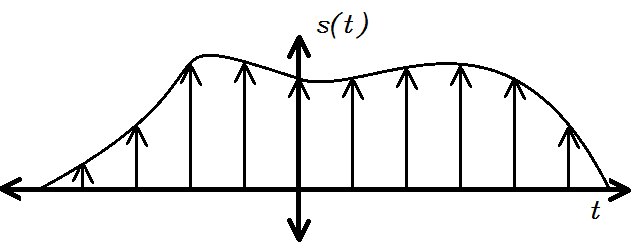
\includegraphics[width=0.5\linewidth]{Pictures/Chapter_2_Lesson_1/Sampling4.png}

So lets assume that we obtain our discrete signal by multiplying our signal with an impulse train:

\begin{equation*}\discFunc(\sampTime) = \contFunc(\sampTime)\cdot\Sh(\frac{\sampTime} {\samplingPeriod})\text{          with \begin{math}\samplingPeriod = \frac{1}{\samplingFreq}\end{math} the sampling period }\end{equation*}

The impulse train is given as a series of delta pulses spaced at Ts:

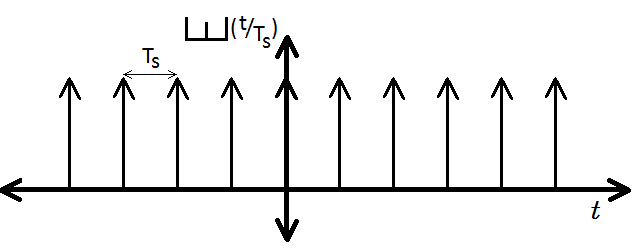
\includegraphics[width=0.5\linewidth]{Pictures/Chapter_2_Lesson_1/Sampling1.png}

So this signal is difined as the sum over infinitely many pulses(delta functions). And the are spaced at a distance of Ts and now here we have multiples of Ts and we have infinitley many that extend into positive and negative time domain.
 
 \begin{equation*}\Sh(\frac{\sampTime} {\samplingPeriod}) = \sum_{\sampIndex}\deltaPulse(\sampTime - \sampIndex\samplingPeriod) \end{equation*}
 
 And now we want to compute the spectrum of this signal.  So to do this we compute the integral over the signal multiplied with the complex exponentials which is basically the definition of the FOurire transform.
 
  \begin{equation*}\fourierSym( \Sh(\frac{\sampTime} {\samplingPeriod})) = \int^{\infty}_{-\infty}\sum_{\sampIndex}\deltaPulse(\sampTime - \sampIndex\samplingPeriod)e^{-jwt}dt  \end{equation*}
 
So how can we solve this integral? Well for instnce by using the sifting property.  This basically states taht if you take the integral of some function f(t) times a shifted impulse, and you integrate over all t, its corresponsd to evaluating the fuinction only at the point T.

\boxed{\int f(t)d(t-T)dt = f(t)\text{      ''Sifting Property''} }

But from because sums and integrals are linear terms, we can shift them.  And then what we get is the sum over infintiely many shifted complex exponential functions:

\begin{equation*}= \sum^{\infty}_{\sampIndex=-\infty} e^{-jw\sampIndex\samplingPeriod} \end{equation*}

So now we have this summation over exponential functions over infinitely many n. So what does this result in.  If I have an exponential function and I sum up over infinitely many n, I will get 0.  Unless wTs  = 0 and multiples of 2pi, because the value of the exponential is one and therefore the summation goes to infinity. SO:

\begin{equation*}= \begin{cases}\infty, & w\samplingPeriod = k2\pi, k \in \mathfrak{Z}.\\ 0, & \text{else}\end{cases} \end{equation*}

SO how can we represent this?  This is is function in spectral domain that is zero everywhere but at certain points it goes to infinity. We can mathematically describe this a a shifted delta function in the spectral domain.

\begin{equation*}= \sum^{\infty}_{k=-\infty}  \deltaPulse(w - k2\pi\samplingFreq) \end{equation*}
\begin{equation*}=  \Sh(\frac{f}{\samplingFreq})\end{equation*}

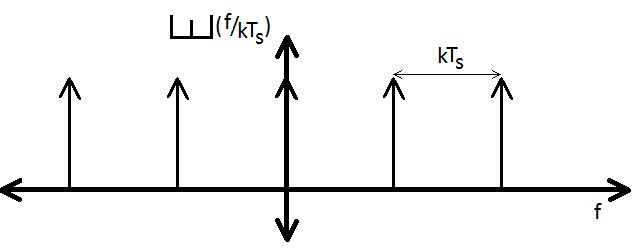
\includegraphics[width=0.5\linewidth]{Pictures/Chapter_2_Lesson_1/Sampling5.png}

So end up with a pulse train in the spectral domain, however the distnace between pusles is no longer the sampling period, but the sampling frequency.  So what have we accomplished here.  We had a continuous time domain signal and we were interested in the resulting spectrum that we obtain when discretize the signal.  We already know that a discrete signal in time domian correpsonds to a periodic signal in frequency domain.  So, but how does it exaclty look and what are the distances between these periodic repetitions, that is something that we just computed cause this distnace will be exaclty the sampling period. SO meaning that in order to compute the spectrum of our signal d(t) what we would need to do is take the fourier transform of our continuous time domain signal x(t) and convoilve it with our impulse response.  Meaning:

\begin{equation*}=\uppercase{\discFunc}(f) = \uppercase{\contFunc}(f)*\Sh(\frac{f}{\samplingFreq}) \end{equation*}

So lets assume X(f) has a certain spectrum something like this:

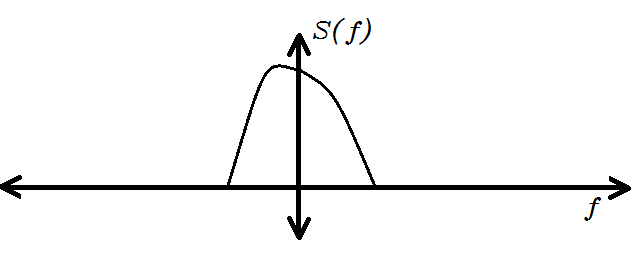
\includegraphics[width=0.5\linewidth]{Pictures/Chapter_2_Lesson_1/Sampling3.png}

and now we convolve this with the fourier transform representaion oif our delta comb

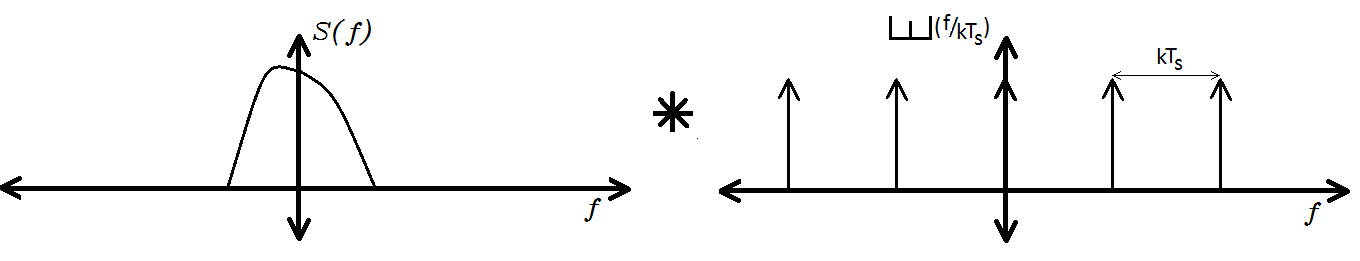
\includegraphics[width=0.5\linewidth]{Pictures/Chapter_2_Lesson_1/Sampling7.png}

SO how would the resulting spectrum look? It would have a periodic representaion.  So what we are drawing here, we can visually derive the sampling theorem.  SO because what happens if we take the sampling frequency too low? If we don not sample our signal often enough.  The replicas of the spectra will overlap meaning that we cannot simply separate the replicas anymore.

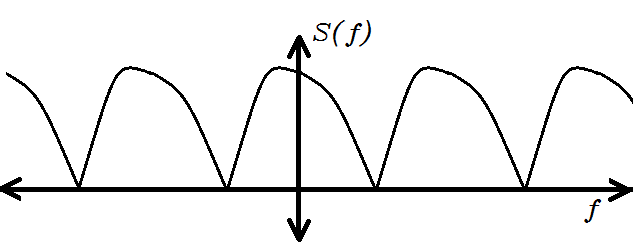
\includegraphics[width=0.5\linewidth]{Pictures/Chapter_2_Lesson_1/Sampling8.png}

SO if fs too low(Ts is too large) then:

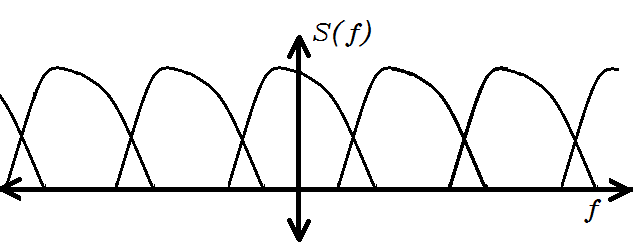
\includegraphics[width=0.5\linewidth]{Pictures/Chapter_2_Lesson_1/Sampling6.png}

 We get our spectrum, except the replicas do not perfectly overlap. This means that we cannot perfectly obtain my signal back again except in trivial examples or specific examples. However, when I have the correctly chosen sampling frequency, then we can simply obtain our signal through lowpass filtering. However this cannot be done when there is an overlap of the signals. SO what does this mean? 
 
 If I choose my smapling frequency, fs, large or equal to 2x's the highest audio frequency, fa. I can perfectly reconstruct the continuous signal x(t) from its discrete representtaion.  
 
 SO this means that if we have a continuous signal, and we sample it with a certain sampling frequency it is true that well you do not sample the samples between two samples. Right so you don not have direct access to these samples, but if the audio bandwidth of this signal is limited it also means that the change between to samples is limited because its a low pass filtered signal in a sense and then if this is the case then you can perfectly interpolate the signal between two samples in a way that you perfectly reconstruct the original continuous signal.
 
 Another way of looking at it or to understand it maybe is that if you have .....what this basically says is that you need a bNDLIMITED SIGNAL that there cannot be a frequency in the signal largeer than fa. that also means that in time domain the change between two samples is limited and so if you fulfill the sampling theorem, you can perfectly reconstruct the signal.
 
 If you obey the Nyquist theorem, tehre is a one to one correspondance between discrete and continuous signals, meaning that we can perfectly reconstruct them.  ANd then if you dont obey it, we get mirror images there will be energy in the signal where it should not be.  If wanted to sample the signal at a lower sample rate, we would need to first apply a low pass.  This would a solution.  Either we could just just a sample frequency high enough, or another thing that we could do if we wanted to choose a lower sample frequency. With speech sounds, we hear these artifacts with high frequency sounds such as s.
 
 SO typical bandwidth that we use.  In telephony, like an ISDN phone but also with your cell phone, we work with sampling rates of about 8khz and then we also low pass filter our signal.  ALthough we have drawn the low pass filter very steep, in practice we cannot realize it this steeply.  So lets say we have speech signals with a bandwidth of up to 16khz.  Then now we use a sampling rate of 8khz, we dont want to havce any information after to 4khz.  But you will not be able to realize low pass filter that has an ideally steep cutoff freequency, but instead, what we would have is something that goes a liitlle more like this... meaning that the spectrum will be distorted up to lower frequencies, and for telephone, the area to where the frequencies are not distorted is 3.4khz. So this is this number here, so theortically speaking, with a sampling frequency of up to 8khz you could recontruct a signal of up to 4khz audio bandwidth, but as you need a vertain lowpass filter that has a certain rolloff the area where the speech is undistorted is only upto 3.4khz.
 
 For music, of course we need higher audio bandwidths,  .....as we said for telephone speech we have 8khz bandwidth, if we have wideband speech telephony, the sampling rate is higher and so the sound quality is better that you can have in a lossless transmission.  Thiese are coding strategies used in some voice over IP clients.  Hifi would be even higher with 44.1kHz, or some standards use 48khz. However at 96khz we are beyond the threshold of hearing and ti makes no sense. 
 
 The next thing that we have to do to discretize a signal, we talked about the discretiaztion on the time axis, but we need to also discrteize the amplitude axis and this.  LATER.
 
 one period no longer fits into one frame  the what happens is, you would basicallc convolve the signal wit ha synch function and you's see samples of the synch function and then you would take discrete samples at theese points.  and then you can imagine that if you have closely spaced sinusoid you will not be able to resiolce those. So a problem is that for the windowed signal, not only do you have one peak at one frequency, you also have what is called spectral leakage so you see energy at frequency components where there is no energy.  and the only way to make this better is to apply tapered anaylsis windows.

For instance a Hamm window or a Hann window because then if you look at the frequency response, you get something that has a certain mainlobe around zero and certain sidebands.  And these sidebands get highly reduced if you tapered analysis window and that basically helps to reduce the spectral leakage effects.  And this is again the same example, the same sinusoid as two slides before and now we see the sinusoid fits the frame length, but still we have a maximum peak where it should be, but you also see that there is energy in the two succesive samples.  SO this is the price that we have t opay for the gain in sideband attenutaion, so you have a wider main lobe meaning that you also have a worsened frequency resolution. SO if you can imagine that if you have a second frequency or a second sinusoid close to it, the frequencies are more likely to mix. But you also see that for a sinusoid that doesnt ideally fit inot the segement, the energy leakage that you would have had a frequencies further away, from the signal frequency would be reduced. 


SO what is the advantage of using such windows? Here you see the time domain window so this is a Hann window this is a Haming window and this is a rectangular window of size 20.  -10 to 10.   so 20ms and here you see its spectral representation where you can see that the higher that this curve is, the more spectral leakage taht we observe and we want to reduce it so we would prefer the red window, the Hann window. However  nothing coes for free. To be able to reduce this spectral leakgae, we also increase the width of the main lobe.  SO here for the rectangular window, its just that steep but the nit does nto reduce that much anymore, but for the other two, for these bell shaped curves, they have a a wider main lobe, but the side band attenutation is increased.  SO somehow we trade off between the spectral resolution awhich is given by the widths of the main lobe and the spectral leakage. SO we can either have a very high spectral resolution with a lot of spectral leakage, or the other way around .  And normally we choose, in a typical situation, the tapered windows.  The rectangualar window is rarely used. 

SPectral Resolution
So the spectral resolution depends on the choice of window, but it also depends on the length of the window.  SO this here, that is the normalized angular frequency its 2pi/N where N is the number of sampüles.  So the length of the window. THe longer the window is so lets say N is very large, then this here the delta phi which is the distacne  between two neighboring bands in frequency becomes much smaller so instead of lets say 200Hz resolution we have 50Hz.  And sometimes you can just take a longer signal if your signal is too short, so we artificailly increase the length of N. How can we do this? Well we take the signal that we have and append a lot of zeros to it.  Thats called zeropadding.  And with that we really increase the number, N so that we increase the number of frequency bins howerver you do not add any addtional infromation, you just add zeros so you do not REALLY increase the spectral resolution but you just increase the sampling. SO here is just ....

so here we have a rectangular window and there are two signals bot consist of two sinusoids with almost the same frequency just a little apart where these two are closer together than these two. YOu can see that for this length, N=16, the DFT is not capable of resolving the two peaks, so what you see when you compute the DFT is 008800008800. You will just see one peak, not two specific ones. While if they are further apart,you can see that these peaks are still resolved.  

so now lets goto zero padding.  So here we have the same signal, but in the lower one, you just increase the number of zeros and what you can see is that the DTFT looks exactly the same, thats the information available in the signal, but its just sampled more often, more frequently so we just sample here, sample there.  So there is no more information, it is just sampled more densely.  Thats the effect of zero padding
% CHAPTER 3 LESSON 3
\clearpage
\section{Discrete Fourier Transform (DFT)}
\label{Discrete Fourier Transform (DFT)}

 The discrete FOurier transform is what we usually work with.  The discrete time FOurier transform that we defined before but the problem here is that if you in  practice you cannot compute it because it is defined as an infinite sum over the signal that you are looking at and in practice you cannot compute an infinite sum, it would take forever literally.  SO what you would have to do is in practice is take a finite time sequence and in a similar way to how we understood sampling again you can think about what does that mean if you chop a certain segment from a signal. And this you can model by multiplying the signal with a rectangular window.
 
 So this would be our time domain signal, with a certain spectrum which can be periodic becasue we have a discrete time fourier transform so this is a discrete signal in time domain giving a continuous and periodic spectrum.  We multiply this with a rectangular window function and this rectangular window function corresponds to a synch function in the frequency domain.  Meaning that if we multiply the two, what you get is a convolutuion of the spectrum with a synch function and this convolution means that you smear your spectrum in the specectral domain,  Meaning that the spectral content will be smeared which also means that your frequency resolution decreases for instance if you have two closely spaced sinuosids and you want to distinguish between them in the frequency domain you need this synch function to be narrow enough so that two signals do not interfere with each other. So lets say 
you have two sinusoidal signals that correspond to two deltas in the spectral domain.  SO we have x1 and x2 which are the sums of two sinusoids. So  now this figure is no longer infintelky log as we would beed it for the discret time FOurier transfom, but we would chop it somewhere.  That means that we will convolve the spectrum with a synch function and then we have a synch function here and a synch function there and you will add the sum of them, meaning that if the synch function gets too broad, then in the resulting spectrum you might get something that looks like this.  Where you are not able to see the two peaks.  This happens if you choose the rectangular window too small.  So in order to increase your spectral resolution you would need more data, in a sense, to find the two sinusoidal components. This is what we learn in this simple example, the trick is that we must know that a multiplecation in the time domain corresponds to convolution in the frequency domain and the fact that a rectangualr function in time domain corresponds to a synch function in the frequency domain .

So now we understand the influence of cutting the spectrum so what do we have here. If we sample the freequency spectrum with sampling period 1/nT then the final time sequence n samples will periodically repeated without and overlap, time domain aliasing. SO what you see here is that the what we are trying to derive here is that the discrete fourier tansform representaion. because in the representaion that we had before, the discret time fourioer  transform,  we had a discrete time representaiton but a continuous frequency representaion now we try to understand what happens if we sample my spectrum, it means that in time domain, my signal will be periodically repeated in the same way that we derived the frequency domain representation and out sampling theorem.

And what this basically means is thta if we discretize oiur spectrum, alos our time domain signal will be repeated and if then also take a rectangular windoww a certain length N, the same way that we did witjh the sampling theorem, we have to take care that when I periodically repeat my spectrum, that these two segments do not overlap. And that correpsonds to how I sample the spectrum in the frequency domain. SO what happens basically, is if you have a discret fourier tansform analysis, that first of allyou look at a windowed part of your time domain signal, then you sample your signal in the frequewncy domain and that corresponds to a periodica represntation of you signal.  If you do use the dft in matlab, then we only look at part of it, the first n sammples both in time domain and in frequency domain, but what you should keep in mind at least in the theory part, that these segemnts will be periodically repeated which is becaue a discrretized signal in time domain correpsonds to a periodic spectrum and a discret frequency domain signal corresponds to a periodic time domain signal. 

And then we have now the discrete fourier transform defintiom where we have bnoth a discrete time domain signal with sample index n and a discrete spectrum with frequency bin index k. And well for the discrete fourier transform, this is what we will mostlay use, for in speech analysis for in this lecture, it'll again have all of these propertioes, Linearity.

In practice, we have fast ways of computing the discrete fourier transform, for instance, the fast fourier transform.  And this is one of the reasons why the discrete fouriertransform is a very often used  spectral representation for speech signals or for audio processing in general  because we have this fast fourier trandform  which is computationally efficient and allows for a fast representaiton of the spectrum of a asignal. And this is one of the basic tools that we use in speech processing. 

Windowing corresponds to the fact that if you chop the signal, it corresponds to the convolution of the function wioth a synch function. For instance, if you have a sinusiod then this would ideally correspond to only one peak in the spectrum, so this  a DFT representaion.  And if the sinusoid fits exactly the window that  youre looking at then also, in the DFT domain, you would see one peak.  Howevre if this is not the case, so again we would have 16 samples inthe time domian, but now the frequency a bit diffeent,
% CHAPTER 4

\setcounter{chapter}{3}
\chapter{Spectral Analysis of Speech Signals}
\thispagestyle{plain}

%Box with Learning objectives should be at the beginning of each chapter
\begin{corollary}

	\hspace*{10mm}
	
	\vspace{5mm} %for optical corrections
	% optionaler Text	
	
	\begin{itemize}
			\item Spectrogram (narrow-band vs. wide-band)
			\item Spectral envelope
			\item Synthesis: Overlap-add technique
			
	\end{itemize}
\end{corollary}

\newpage

% CHAPTER 4 LESSON 1
\clearpage
\section{Spectrogram (narrow-band vs. wide-band)}
\label{Spectrogram (narrow-band vs. wide-band)}

 So what we now would like to do is apply the concept of the DFT and the fourier transform to speech signals and for that we first have to analyze the speech signal and then typically, some modification is done and then we must synthesize it again.
 
 The one tool that we use most frequently in audio processing to analyzse the spectral content is the short time fourier snalysis so what is the idea behind it?  Well its speech signals, like what I am saying right now is time varying, so an A is very different from  a ssss so we can't just take one speech utterance and compute the DFT of it and work with it because it is very different and you want to also see how the frequency content changes over time. FOr that we just have to split the signal into short segments and analyze each of them more or less independently of each other. So we can see how this spectral content changes over time. And we do this by means of the STFT. and basically all of the considerations that we did before still hold for the STFT and there are a set of parameters that you can choose for the STFT computation and they alwys depend upon what we want to use it. 
 
 So here is one example a chirp. A decreasing frequency and the na splash at the end. So these two signals are very different over time. If we were to compute the DFT of each part, they would look astonishinly the same.  Becasue here there is energy in high frequency decreasing in time.  If we were to take the mean over the time, the result would be similar to the splash.  So if we were to see the DFT of each part it would be hard to see what the underlying time domain signal would look like.  Therefore we do this analyis wher we can also see how it changes over time.  In this visulalization we can see how the chirp is time varying whereas the splash is broadband over time and is very different. 
 
 SO this is how we comput the STFT. Lets first see the analyis part of it. We use the sliding window transform.  We have a long speech signal and instead of taking one DFT of it we would rather take pieces. And for each segment, we apply the DFT.  But we learned some tricks before we apply the DFT.  We first apply an analysis window.  We could just cut it out and that would apply to having just a rectangular window or we could apply a Hann window for example to improve the spectral content or to reduce the spectral leakage.
 
 This can mathematically be stated this way, where the w is the analysis window of length N. l is the fram index and basically what you do is you have the window here and you multiply it with a shifted version of the original signal to get the current signal segment xl.  And there are some values here.  There is a window length N, a local time index starting a 0 and going to N-1, and there is a n overlap of these signals which in the way I drawed it there its about 50\%.  So each of these  time domain signal segemtns that are weighted with a window for them, the DFT is computed in that way.
 
   This is the typical formulation of the DFT. And its complex valued.  And these are the so called STFT coeffcient wher k is the frequency index and l is the frame index.  So for every frame we have some frequency bands.
   
   And here is one example of it.  Here is the chirp signal with the frequency increasing. A single tone sinusoid with increasing frequency and these two bell shaped curves represetn the analysis windows.  And then we apply the window and compute the DFT and that is what we get. This is however a diffuclt way of visualizing the result, so we use a spectrogram
 
 So there we have a two dimensional representation where we have on the xaxis, the time or the segemnt index and on the yaxis theres a frequencyand the actually amplitude of the magnitude is coded in color. So only the amplitude is considered, most of the times, the phase is not considered. So we limit ourselves to magnitude.
 
SO that is one spectrogram, but we learned that we have a lot of parameters to play around with, so its a choice of the window, the length of the window, also the overlap and we'll change some parameters. SO right now we have 16khz sampling frequency that has a bandwidth of 8khz and now lets change the size of the window from 512 to 32. What would you expect to change in the spectrogram.  Instead of using a rather long window, we use a rather short one SO you use a short window, you only use short segements, and you update them quite often so you have a high temppral resolution. However we learned that the resolution is 2pi over N. So we decrease N and the resolution in the frequency domain reduces. So we can either have high temporal resolution for short windows or have a bad resolution in the frequency domain or the other way around.  Have a long window, a high end, meaning a good resolution in the frequency domain, but we can't tract changes in the time domain signal that fast anymore. SO lets see what happens when we use such a short window.  It looks like this, you can see that where we were capable of resolving the harmonics, we are not capable of that anymore but you can see changes in energy very decently and you can even see like here you see these horizontal lines are not constant but now there is little energy, lot of energy, little energy that really depends how this fram lies relative to the frequency. What part of the sinusoid it is cutting out.  Although for this time here, the energy is rather constant, you have the long one, if you only use the short windows its high and then low again, high and then low again. Thats what you see here in the horinzontal lines.

So lets do the opposite, lets go for very long windows, lets say 2048.  Now we can see that its temporally smeared, but the spectral resoultion is quite high. You can even read it here.  So now lets see what zero padding does.  We leave the window length at 64, but change the STFT to 1024.  This is basically zero padding of 960.  We increase the N, meaning we increase the delta omega, but we learned that this will not increase the spectral resoulton.  Because we are just adding zeros, we should still not be able to resolve the harmonic components. Basically its just more less rough, more smooth picture, So a bit like interpolation in between but its not adding any new information to it. So now lets not do zero padding, but use a window length of 1024, now you can see that we are indeed capable of resolving the harmonic components. Then maybe one other example that we could have a look at, lets change the window function that we use so, its the Hamming window, lets take the Hann window.  SO you can see that there are minor changes in it because they basically look very much alike.  And now lets take the rectangular window and you can see that it looks like this . We can see the spectral leakage, everything is a bit blurred do to the spectral leakage. We change the window and we can see that we are back to normal again.

The resolution problem is limiting. YOu jkust have tolive with it.  and  you always have to find the best trade off for your application so if you want to like, if you have a fastly changing signals like a plosive that is very short then maybe it would be nice to use short windows, but like for an aaaaa that is very stationary, you can use longer windows and everything is alirigth.  It is always depending on the application.  Typical choices of window length are 20-30 ms.  Becasue you can assume most speech sounds to be rather stationary for segment length of upto 30ms that a rulle of thumb.  

SO here is an example for a wideband spectrogram, that is a spectrogram using short segements having a not so good frequency resolution.  And here is just the setup so for this picture here we used a window length of 5ms and window shift of 2.5ms which is an overlap of 50\% and we could, what I also showed in the program, is that we could also increase the FFT length, we add zeros at the end of the signal but we dont get any additional information but it looks nicer. These windows could rather well represent plosive sounds however the spectral resoultion is not good enough to resolve the harmonic structure of voiced speech.  Okay and here is the opposite of it.  A narrowband spectrogram. where we use longer segements. 32ms.  Window shift is also 50\% but you could also reduce it a bit more if you wanted. It decreases the computational load and gives a bit nicer piuctures.  It has rather long windows so it is not so good at tracking fast changing signals, but its good for rather stationary signals where you can allow rather long windows.  So here is a pictrure showing both spectrograms at the same time so they are the same signals.  Here is the narrowband, so good frequency resolution, and the wideband spectrogram where you can see what we already discussed. 


Slice Computation

Thats basically one conclusion slide. Thats for a typical setup, lets say 32ms, thats a rather good compromise its rather on the long side., but its still okay.  And we use frame shifts that correspond between 50 and 75 percent, sometimes even more and we use overlapping frames. and why that is I will be explaining in a few slides. And what we can also do is preemphasis.  Acoustic sounds in nature always obey a 6dB attenunation per octave, so towards higher frequencies, there is always an attenuation and that is is not a proble, but for visualization, this can be not to good. So therefore we can apply a highpass filter first wchich boostst the higher frequencies so that we get a bit nicer picture.  So this is only for visualization.  Normally this is not done for the modification, the actual processing. SO here there is no preemphasis on it, and now lets add some emphasis to the higher frequencies. Lets say 0.99. So now we can see that the higher frequencies are a bit more pronounced as before. 
So after splitting the signal into segement and maybe preemphasizing the signal, then the window is pllied to improve the spectral behavior and then we are basically done with the spectral analysis.
   
% CHAPTER 4 LESSON 2
\clearpage
\section{Spectral Envelope}
\label{Spectral Envelope}


Envelope

So here we have one speech sentence.  And we pick put three representative segments. WHich is an f, an i, and an u. and we have a look at the spectrum, the DFT of the short signal segments. And you can see that for the f there are rather high frequency spectral components, but for the i and the u you see the formant structure, but also the fundamental frequency in it that you cant see for the f because there is no fundamental frequency. SO these, the envelope between f, i, and u is rather different.  So lets see how closely they are realted to each other for the same vowels, The same sound.  SO there are three segemnts taken from the same u and you can see that these spectra look rather alike. So not the spectra itself, but the envelope. They are rather similar, so as I said before, the envelope is basicall what we do with our vocal tract and this carries the information so if the envelope looks more or less like this then it will sound like a you, while the envelope her in blue would sound like an f.  SO how do obtain the envelope?  Well it would be possible to just look at the wideband spectrogram and you basically have the envelope already.  But it changes rather quickly, so here  these horizontal lines, its more energy, less energy, more energy, so its not very robust, so there are more advanced techniques like LPC,Cepstrum)  The bottom line here is that most of the time, we will be using narrowband analysis, meaning that we use signal segments between 16 and 32ms and we will obtain the spectral envelop not from the wideband, spectrum, but via other methods that will be coming later.

% CHAPTER 4 LESSON 3
\clearpage
\section{Synthesis: Overlap-add technique}
\label{Synthesis: Overlap-add technique}

The typical way that we work with signals in the frequency domain is that we first analyze it. Then we do some modifications to it, lets say we have a noisy signal, lets say there was some construction work noise and we want to get rid of it, so we want to apply noise reduction, or we want to reduce echos if the are undesired, or we could stretch the signal in time or do pitch shifting and once we are done with all of these modification, we have to synthesisze the time domian signal again because we can only listen, our loud speaker is only capable of reproducing time domain signals. Thats the reason why we have to get back to time domain. So what we do is ...

We first take the segement, the overlapping segments, we apply a window again so its a lot of repetition and then compute the DFT. So lets say this is the analysis window here, we do some magic in the modification step and then we want to go back so we apply the inverse DFT. SO if there is no modificaltion, we have w(n)times xl(n). So this small part of the whole signal x is called xl.  So we bring it to the DFT domain then we directly bring it back to the time domain, so we have w(n)*xl(n). SO we basically have these signals again. SO in the next step we have to get back to our time domain signal because right now we just have these separate segment. SO now we align them in the same way that we took them out of the singal, so overlapping lets say by 50 percent and then we add them up.  And then come out with something that basically looks like this.  SO they should ideally always add up to one, these windows.  Becasue in case that they would not do it, we would not have what we call perfect reconstruction. So what we want to have is apply the STFT then the inverse STFT and then we get exactly the same signal back gain. And this is only possible if this addition here, this signal sums up to x(n) again up to some offset, lets call it delta. So the most, the onlydifference that should be between that one and the original signal should be one offset here, one time domain offset. Not more than that.  That is something that we are definitely aiiming for. 

ANd for that the windows and the overlap need to fulfill a specific relation. Mathematically we can state it like this :
So yl(n) is the windowed segemtn, x(n) is the segemnt wihtout a window. And w(n) is our analysis window. And we bring it to the DFT domain and back to the time domain .  ANd then we apply a synthesis window.  Synthesis window I did not introduce yet, I will talk about that shortly, but lets for now assume that we need a synthesis window that is after the DFT and the IDFT. We aplly another windo which is called v(n) soin the end. We have something that is:

So mathematically, we can say that this summation here should always be one, that is what I tried to draw there and here are some examples of that.  Here we don not apply a synthesis window and we just take v(n) to be one(rectangular), so then this formula on the bottom right reduces to that one so that the analysis window should add up tot a constant value, so here we use a triangular analysis window, a hamming window and and Hann window and you can see that if you add them all up one after the other in thhis overlap fashion the nyou end up with a constant value here.  SO this is just like boundary issues, in the very beginning and in the very end but in between tehre should be always one. But that is not guarateed all of the time.  SO lets say here, we take a Hann window for example, in this case it adds up to 2, this is an overlap of 75percent it adds up exactly to 2, thats nice.  But you could also have it that this is not the case like if you had a strange overlap of 30 percent or something.  Then this would not add up to one any more but would add up to something like this. So this would result in modulations in the reconstructed signal that are not desired.  SO its not the same window that we put into there anymore.  So for lets say for a Hann and Hamming window toachieve perfect reconstruction we need overlaps of 50 percent, 75 percent, 87 percent.  The shift needs to always be at 2 to the power of -somehting to be accurate.  You always have to take care that your choice of window length, shift and the form of window are such that it allows for perfect reconstrucution. 

So the most frequently used one is 50 perccent, because if you use 75 percent you have double the numberof segement s that you have double the computational load that you need to process it and in our area, lets say we goto hearing aids and computtauonal load is extremely important becasue we only have a short battery life and for hearing aid users to accept a hearing aid, it needs to run a t least a week without changing the battery. so you really need to take care about power consumption.

So now we come to the synthesis part and go more into detail becasue now we assum that we have done something to the signal.  Upto now we have only go in and out, but lets say we did do some modifications to it. So thats a segment, and then we apply a Hann window to it, then we bring it to the frequency domain then we do some modification, lets say we multiply it with some function Gomega()and multiply it with the windowed function Xw(omega) and go back to time domain. In the case that G is one, then we would get the same signal, everything is fine again, no problems at all.  And but in the case that we apply some G here that is a multiplecation in the frequency domain, so we get a conviltuion in the time domain. SO lets say this one here, if you bring it to the time domain is g(n), and output is something that is g(n)convolved with x(n)w(n).  Its not the same signal anymore, but its also what we are aiming at. Lets say the g looks something liek this and we convolve this with the original signal here. And what would happen is herer(beginning ) the values would be different from zero and the output would look something liek this, and you cannot see the window anymore. Ans this could be problematic, becasue here you have these boundaries, and boundaries are always bad, so if you start overlapping and adding them again, then you have here some parts where it is not zero and the other part is the same and when they add up, you might end up with some artifacts that are audible. and that you dont want to have.  And this is the reason that we often apply a synthesis window.SO after all of this processing, we again apply a window that looks something like a Hann window, to reduce these boundary issues here. And with that, we reduce the audible artifacts.  Thats one solution to the problem, another solution could be that we use an analyis window, but apply zeropadding.  That could also help. 

Lets say g has a length Lg, and x(n)(w) has a length of N.  SO if you convolve two signals of these length, the length is L+N-1. And this is longer than just N. So there could be something like this there, but since it is not therre, we fight with circular convolution, the stuff thats in a linear convolution would show up here, shows up here again(beginning) and this is what is coming up in this area here and  this is what produces these artifacts. So lets now again ask the question, why would zero padding help to avoid that. So basically the additional length of the signals is all zeros but that really depends on g, that can be really long, 

So these two ways exist, so you either append zeros here or you apply a synthesis window at the very end, where the synthesis window is also just an approximation solutionto it becasue we still see some of the errors in there, but they are reduced.  The synthesis window has the benefit that it introduces minimal computational costs. WHile here, adding zeros to it introduces additional costs in computing the STFT, then there are more frequency bands in the STFT and there is more computational overhead. 

And how can we choose the synthesis window. One typical choice is the square root Hann window. So we said that for a 50percent overlap, the Hann window produces perfect reconstruction of the original signal if we don not apply any modifications here. However, if we apply a synthesis window here, then by using the Hann window afterwards again a different window, would not be capable of producing perfect reconstruction anymore.  SO what we need is not that w(n) allows for perfect reconstruction, but w(n)v(n) so the multiplecation of the analysis window and the synthesis window that is basically, applied.  These two need to allow for perfect reconstruction and we said that if v(n) is one, then we can use the Hann window for w(n), but another choice is that we use the square root of Hann here and the square root of Hann there and  that allows for perfect reconstruction.




% CHAPTER 5

\setcounter{chapter}{4}
\chapter{The Vocal Tract and Linear Predictive Coding}
\thispagestyle{plain}

%Box with Learning objectives should be at the beginning of each chapter
\begin{corollary}

	\hspace*{10mm}
	
	\vspace{5mm} %for optical corrections
	% optionaler Text	
	
	\begin{itemize}
			\item Tube Model of the Vocal Tract
			\item Linear Prediction
			
	\end{itemize}
\end{corollary}

\newpage

% CHAPTER 5 LESSON 1

\section{Tube Model of the Vocal Tract}
\label{Tube Model of the Vocal Tract}


The first chapter introduced the concept of the source filter model for speech production. In this model an excitiation source (air pushed from the lungs) is passed through a filter (the vocal tract) to produce speech. Air pushed from the lungs can be periodically regulated by the glottus producing a voiced speech sound.  When the glottus is not used, and air is simply pushed through the vocal tract, an unvoiced sound is produced. Because the vocal tract is not perfectly cylindrical, reflections occur. These reflections produce resonances, also called formants, that are critical for distinguishing speech sounds. 

\begin{figure}[h]
	\centering
	 \def\svgwidth{10cm}
	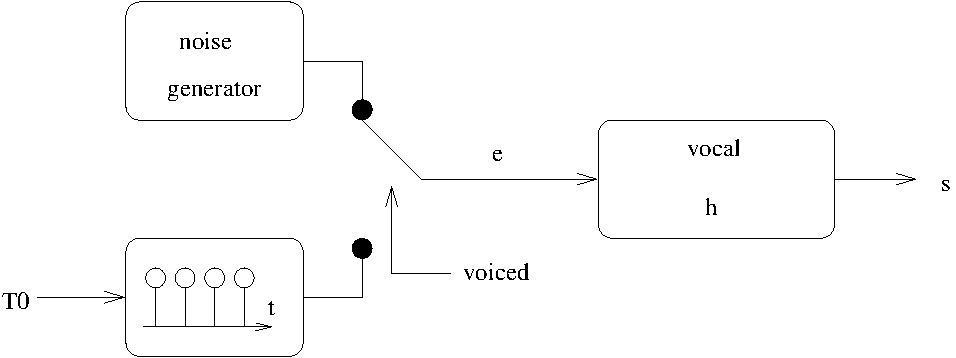
\includegraphics[width=0.5\linewidth]{Pictures/Chapter3_Lesson3/filterVUv2-eps-converted-to.pdf}
	\caption{Source filter model of the vocal tract}
	\label{fig:SourceFil}
\end{figure}

Figure 3.1 displays the method that will be sued to model the excitation sources. Voiced speech is modelled as a pulse train, whereas random noise is used to model unvoiced speech.  Note that there is a switch in the diagram implying that the model will require some sort of detection to switch between the two sources. 

Now we want a model for speech production.  We therefore decompose speech into excitation souorce and spectral shape. The excitation source can be modelled as a pulse train. Unvoiced can be a random noise generator.  Also can be used for mixed excitiation. 

The second part is the vocal tract filter that can be modelled by a tube where we ignore the nasal tract because it is complicated.

What we want is a mathematical model for the vocal tract. Once we have this model, then we can estimate the parameters that describe the shape of our voacl tract only from the speech recording. We start with what is phsically going on in the vocal tract.

We know that sound is a pressure wave.  That there air particles in it that oscillate back and forth.  There are area of compression and areas of refraction.  

WE now consider a pressure wave within a tube.  The interaction of the particles with the tube ends whteher open or closed introduces boundary conditions to the problem, that affect the propagation of the wave through the medium.  At the open end the pressure wave is forced to have a minimum, at the closed end, it is forced to have a maximum.

We define pressure P(x,t), v(x,t) V(x,t) from these, we can define an acoustical impedance.

Whenever there is a change in impedance, we have a reflection.  This can be charaterized by a reflection coefficient that is a function of the acoustical impedance of the two media.

Put in equations

The close end = pressure maximum, velocity minimum (particles cant move.)
open end = opposite

put into equations we see that

 at the closed end, the reflection coefficient goes to -1

at the open end, we have a reflection with +1

This now implies that we have a backward travelling wave from the open end reflection.  The forward wave and the backward wave will add up. They will add up if they match the resonance frequency of the tube. 

picture of tube with wavelengths.  Derivation of equations for vocal tract resonances. One resonance per kHz!!!! Approx 4 resonances per kHz. However if this was the case with our vocal tract, speech would be unintelligible because the formants do not change.  Becasue we cannot alter the length of our vocal tract, we can instead constrict certian parts to change the postion of the resonances. We have to therefore model the voacl tract as a tube with individual segments that change their shpae over time.

pictiure

We can treat this as a set of short indivudal tubes and do the same computations for each segment as we did for the tube.  We can then concatenate the results to get our filter.

SO we have short cylindrical tubes with different areas 

equations

Assumptions:
low friction, plane wave prop

Therefore we can use equations for pressure and volum velocity 


% CHAPTER 5 LESSON 2

\newcommand{\indexTime}{n}
\newcommand{\convIndex}{m}
\newcommand{\excitationFunc}{e}
\newcommand{\filterFunc}{h}
\newcommand{\filtOutFunc}{s}
\newcommand{\predictionError}{d}
\newcommand{\Error}{E}
\newcommand{\newIndex}{\mu}
\newcommand{\autoCorr}{\phi_{s}}
\newcommand{\maConvIndex}{m}
\newcommand{\arConvIndex}{\nu}
\newcommand{\maFiltOrder}{q}
\newcommand{\arFiltOrder}{p}
\newcommand{\maFiltCoef}{b}
\newcommand{\arFiltCoef}{a}


\section{Linear Prediction}
\label{Linear Prediction}


\begin{itemize}

\item Goal: Find a model for the vocal tract filter from a speech signal.

\item In general, this filter can be modelled as infintitely long

\begin{equation}\filtOutFunc(\indexTime) = \sum^{\infty}_{\convIndex = 0} \filterFunc(\convIndex)\excitationFunc(\indexTime-\convIndex)\end{equation}

\item The infinite sum can be replaced by a finite recursive equation.
ARMA model 

\begin{equation}\filtOutFunc(\indexTime) = \sum^{\maFiltOrder}_{\maConvIndex = 0}\maFiltCoef_{\maConvIndex }\excitationFunc(\indexTime-\maConvIndex) -  \sum^{\arFiltOrder}_{\arConvIndex = 1}\arFiltCoef_{\arConvIndex }\filtOutFunc(\indexTime-\arConvIndex)\end{equation}

\begin{equation}\MakeUppercase{\filtOutFunc}(z) =\MakeUppercase{\excitationFunc}(z) \sum^{\maFiltOrder}_{\maConvIndex = 0}\maFiltCoef_{\maConvIndex }z^{-\maConvIndex} -  \MakeUppercase{\filtOutFunc}(z) \sum^{\arFiltOrder}_{\arConvIndex = 1}\arFiltCoef_{\arConvIndex }z^{-\arConvIndex}\end{equation}

\begin{equation}\MakeUppercase{\filtOutFunc}(z)(1 +  \sum^{\arFiltOrder}_{\arConvIndex = 1}\arFiltCoef_{\arConvIndex }z^{-\arConvIndex}) =\MakeUppercase{\excitationFunc}(z) \sum^{\maFiltOrder}_{\maConvIndex = 0}\maFiltCoef_{\maConvIndex }z^{-\maConvIndex} \end{equation}

\item In the Z domain, we can define the transfer function 
\begin{equation}\MakeUppercase{\filterFunc}(z)  = \frac{\MakeUppercase{\filtOutFunc}(z)}{\MakeUppercase{\excitationFunc}(z)} = \frac{ \sum\limits^{\maFiltOrder}_{\maConvIndex = 0}\maFiltCoef_{\maConvIndex }z^{-\maConvIndex}}{\sum\limits^{\arFiltOrder}_{\arConvIndex = 0}\arFiltCoef_{\arConvIndex }z^{-\arConvIndex}}     |_{a_0 = 1}\end{equation}



\begin{itemize}
\item Transfer function consists of two polynomials-

\item Fundamental theorem of algebra

\begin{itemize}

\item  ''Every non-zero single variable polynomial has at least one root.''  polynomial of order n has n roots

\item A polynomial in z can be divided by (z-a)

\begin{itemize}

\item \begin{equation*}  \frac{p(z)}{(z-a)} = q(z) + \frac{R}{z-a}\mbox{\begin{math}\implies\end{math} R: not a function of z}\end{equation*}

\item \begin{equation*}p(z) = (z-a)q(z) + R\mbox{\begin{math}\implies\end{math}q(z) is a polynmomial w than p(z)}\end{equation*}

\item if \begin{math} a = z_0\end{math} is a root, then
\begin{equation*}p(z_0) = 0 =  (z_0-z_0)q(z) + R\mbox{ \begin{math}\implies\end{math}  R = 0}\end{equation*}

\item  if \begin{math} a = z_0 \implies\end{math} is a root, then the residual is zero

\end{itemize}
\item \begin{math}\implies\end{math}  Every polynomial can be factorized by its roots
\end{itemize}
\end{itemize}


\item \begin{equation*}\MakeUppercase{\filterFunc}(z)  = \frac{\MakeUppercase{\filtOutFunc}(z)}{\MakeUppercase{\excitationFunc}(z)} = \frac{\sum\limits^{\maFiltOrder}_{\maConvIndex = 0}\maFiltCoef_{\maConvIndex }z^{-\maConvIndex}}{\sum\limits^{\arFiltOrder}_{\arConvIndex = 0}\arFiltCoef_{\arConvIndex }z^{-\arConvIndex}}     |_{a_0 = 1} =\frac{\maFiltCoef_0z^{-\maFiltOrder}}{z^{-\arFiltOrder}}\frac{z^{\maFiltOrder}+\frac{\maFiltCoef_1}{\maFiltCoef_0}z^{\maFiltOrder-1}+...+\frac{\maFiltCoef_{\maFiltOrder}}{\maFiltCoef_0}}{z^{\arFiltOrder}+\arFiltCoef_1z^{\arFiltOrder-1}+...+\arFiltCoef_{\arFiltOrder}} = b_0\frac{z^{-\maFiltOrder}}{z^{-\maFiltOrder}}\frac{\prod\limits^{\maFiltOrder}_{\maConvIndex=1}(z - z_{0_{\maConvIndex}})}{\prod\limits^{\arFiltOrder}_{\arConvIndex = 1}(z - z_{0_{\arConvIndex}})}\end{equation*}

\begin{equation*}\mbox{\begin{math}z_{0_{\maConvIndex}}\end{math}: Roots of numerator polynomial  \begin{math}\implies\end{math} zeros of \MakeUppercase{\filterFunc}(z)}\end{equation*}

\begin{equation*}\mbox{\begin{math}z_{0_{\arConvIndex}}\end{math}: Roots of denominator polynomial  \begin{math}\implies\end{math} poles of \MakeUppercase{\filterFunc}(z)}\end{equation*}

\item{pole/zero model (Z-domain) \begin{math}\rightleftharpoons\end{math}ARMA model (time-domain) }

\begin{itemize}

\item MA process / all zero filter

\begin{equation}\filtOutFunc(\indexTime) = \sum_{\maConvIndex = 1}^{\maFiltOrder}\maFiltCoef_{\maConvIndex}\excitationFunc(\indexTime - \maConvIndex)\mbox{ \begin{math}\rightarrow\end{math}time domain}\end{equation}

\begin{equation}\MakeUppercase{\filtOutFunc}(z) = \MakeUppercase{\excitationFunc}(z)z^{-\maFiltOrder}\maFiltCoef_0 \prod\limits^{\maFiltOrder}_{\maConvIndex=1}(z - z_{0_{\maConvIndex}})\mbox{\begin{math}\rightarrow\end{math}frequency- domain}\end{equation}

\item AR process/all pole filter

\begin{equation}\filtOutFunc(\indexTime) = \maFiltCoef_0\excitationFunc(\indexTime) - \sum_{\arConvIndex =  1}^{\arFiltOrder}\arFiltCoef_{\arConvIndex}\filtOutFunc(\indexTime - \arConvIndex)\mbox{ \begin{math}\rightarrow\end{math}time domain}\end{equation}

\begin{equation}\MakeUppercase{\filtOutFunc}(z) = \MakeUppercase{\excitationFunc}(z)\maFiltCoef_0 \frac{z^{\arFiltOrder}}{\prod\limits^{\arFiltOrder}_{\arConvIndex=1}(z-z_{0_{\arConvIndex}})}\mbox{\begin{math}\rightarrow\end{math}frequency- domain}\end{equation}

\end{itemize}

\item This recursive structure resembles the recursive structure obtained from the tube model. (Nasal tract, glottal and labial filter neglected)

\begin{itemize}

\item The amplitude characteristics can be apporximated by increasing AR filter order

\item We are less sensitive to phase as compared to amplitude changes

\end{itemize}

\item Advantages of the AR Model

\begin{itemize}

\item Always invertible if stable

\item Coefficients can be efficiently obtained

\end{itemize}

\end{itemize}


\subsection{Computation of AR coefficients}

AR Model
\begin{equation}\filtOutFunc(\indexTime) = \maFiltCoef_0\excitationFunc(\indexTime) - \sum_{\arConvIndex =  1}^{\arFiltOrder}\arFiltCoef_{\arConvIndex}\filtOutFunc(\indexTime - \arConvIndex)\end{equation}

\begin{itemize}

\item Successive speech samples are correlated

\item at time n, \filtOutFunc(\indexTime) can be predicted up to the innovation, \begin{math}\maFiltCoef_0\excitationFunc(\indexTime)\end{math}.

\begin{equation*}\mbox{Prediction: }\hat{\filtOutFunc}(\indexTime) = - \sum_{\arConvIndex =  1}^{\arFiltOrder}\hat{\arFiltCoef_{\arConvIndex}}\filtOutFunc(\indexTime - \arConvIndex)\end{equation*}

\begin{equation*}\mbox{for \begin{math}\hat{a_{\arConvIndex}}=a_{\arConvIndex}\end{math} we can predict the speech signal up tot he scaled excitiation}\end{equation*}

\begin{equation*}\predictionError(\indexTime)=\filtOutFunc(\indexTime)-\hat{\filtOutFunc}(\indexTime)=\maFiltCoef_0\excitationFunc(\indexTime)  \end{equation*}

\item find MMSE optimal parameters  \begin{math}\hat{a_{\arConvIndex}}=a_{\arConvIndex}\end{math} by minimizing the mean of the squared error signal

\begin{equation*}\mbox{Approach: Minimize}\MakeUppercase{\excitationFunc}(\predictionError^2)\mbox{How? Set the first derivative to zero}\end{equation*}

\begin{equation*}0 \stackrel{!}{=} \frac{\partial\Error(\predictionError^2(\indexTime)}{\partial\hat{a_{\arConvIndex}}} \stackrel{chain rule}{=}\Error(2\predictionError(\indexTime)\frac{\partial}{\partial\hat{a_{\arConvIndex}}}(\filtOutFunc(\indexTime) + \sum_{\arConvIndex =  1}^{\arFiltOrder}\hat{\arFiltCoef_{\arConvIndex}}\filtOutFunc(\indexTime - \arConvIndex))\end{equation*}

\begin{equation*} = \Error(2\predictionError(\indexTime)\filtOutFunc(\indexTime - \arConvIndex))\end{equation*}


\begin{equation*}=2\Error((\filtOutFunc(\indexTime) + \sum_{\arConvIndex =  1}^{\arFiltOrder}\hat{\arFiltCoef_{\arConvIndex}}\filtOutFunc(\indexTime - \arConvIndex))\filtOutFunc(\indexTime - \arConvIndex))\end{equation*}


\begin{equation*}= \Error(\filtOutFunc(\indexTime)\filtOutFunc(\indexTime - \arConvIndex))+  \sum_{\newIndex =  1}^{\arFiltOrder}\hat{\arFiltCoef_{\newIndex}}\filtOutFunc(\indexTime - \newIndex)\filtOutFunc(\indexTime - \arConvIndex) \end{equation*}

\begin{equation*}\autoCorr(\arConvIndex) =  \Error(\filtOutFunc(\indexTime)\filtOutFunc(\indexTime - \arConvIndex))\end{equation*}


\begin{equation*}=\autoCorr(\arConvIndex) + \sum_{\newIndex =  1}^{\arFiltOrder}\hat{\arFiltCoef_{\newIndex}}\autoCorr(\arConvIndex -\newIndex) \end{equation*}


\begin{equation*}\mbox{Second Derivative}\end{equation*}


\begin{equation*} \frac{\partial^2\Error(\predictionError^2(\indexTime)}{\partial\hat{a_{\arConvIndex}}^2}=\Error(2\autoCorr(0))\geq 0 \rightarrow minimum\end{equation*}

\item Solution to all \begin{math}\hat{a_{\arConvIndex}}\end{math} Wiener Hopf equations/Normal equations. Write in matrix form.

\begin{equation*}\autoCorr(\arConvIndex)=-\sum_{\newIndex =  1}^{\arFiltOrder}\hat{\arFiltCoef_{\newIndex}}\autoCorr(\arConvIndex -\newIndex)=-(\autoCorr(\arConvIndex-1)\hat{a_1} + \autoCorr(\arConvIndex-1)\hat{a_1} + \autoCorr(\arConvIndex-2)\hat{a_2} + \dots +\autoCorr(\arConvIndex-\arFiltOrder)\hat{a_\arFiltOrder} )\end{equation*}

\begin{equation*}\begin{pmatrix}
\autoCorr(1) \\ \autoCorr(2) \\ \vdots \\ \autoCorr(\arFiltOrder)
\end{pmatrix}=-\begin{pmatrix}\autoCorr(0) & \autoCorr(-1) & \autoCorr(-2) & \ldots & \autoCorr(1 -\arFiltOrder) \\
\autoCorr(1) & \autoCorr(0) & \autoCorr(-1) & \ldots & \autoCorr(2 -\arFiltOrder) \\
\vdots & \vdots & \vdots & \ddots & \vdots \\
\autoCorr(\arFiltOrder-1) & \autoCorr(\arFiltOrder-2) & \autoCorr(\arFiltOrder-3) & \ldots & \autoCorr(0)\\ \end{pmatrix}\begin{pmatrix}\hat{\arFiltCoef}_1 \\ \hat{\arFiltCoef}_2 \\ \vdots \\ \hat{\arFiltCoef_{\arFiltOrder}}\end{pmatrix}\end{equation*}

\begin{equation*} \mathbf{\autoCorr} = -\mathbf{R_s}\mathbf{\hat{\arFiltCoef}}\end{equation*}

\begin{equation*} \mbox{Solution to the Wiener Hopf equations gives MMSE-optimal linear predictive coefficients} \hat{\arFiltCoef_\arConvIndex}\end{equation*}

\begin{equation*} \implies \mathbf{\hat{\arFiltCoef}_{opt}}= -\mathbf{R_s}^{-1}\mathbf{\autoCorr} \end{equation*}

\item In Practice: Speech is only short time stationary
\begin{itemize}
\item Estimate autocorrelation on short segements

\item Use temporal averaging instead of E{}
\end{itemize}

\begin{equation*} \mbox{In the so called autocorrelation method,} \mathbf{R_s} \mbox{is estimated on short framed segents } \widetilde{s} \end{equation*}

\begin{equation*}\widetilde{\autoCorr}(\arConvIndex)=\sum^{n_t}_{n = n_1}\widetilde{\filtOutFunc}(\indexTime)\widetilde{\filtOutFunc}(\indexTime - \arConvIndex)\end{equation*}

\item the estimate is symmetric \begin{math}\hat{\autoCorr}(\arConvIndex) = \hat{\autoCorr}(-\arConvIndex)\end{math}

\item the correlation matrix estimate \begin{math}\mathbf{R_s}\end{math} is symmetric and Toeplitz

\item fast solutions (Levinson-Durbin recursion)


\end{itemize}

% CHAPTER 6
\setcounter{chapter}{5}
\chapter{Cepstrum}
\thispagestyle{plain}

%Box with Learning objectives should be at the beginning of each chapter
\begin{corollary}

	\hspace*{10mm}
	
	\vspace{5mm} %for optical corrections
	% optionaler Text	
	
	\begin{itemize}
			
			\item Cepstrum
			\
	\end{itemize}
\end{corollary}

\newpage

% CHAPTER 6 LESSON 1

\newcommand{\indexTimeCep}{n}
\newcommand{\filtInCepFunc}{x}
\newcommand{\filtOutCepFunc}{y}
\newcommand{\filtFunc}{h}
\newcommand{\freqIndex}{e^{j\omega}}

%Einfuhrung in das Kapitel

\begin{equation*}\filtOutCepFunc(\indexTimeCep) = \filtInCepFunc(\indexTimeCep)*\filtFunc(\indexTimeCep)\end{equation*}

\begin{equation*}\MakeUppercase{\filtOutCepFunc}(\freqIndex) = \MakeUppercase{\filtInCepFunc}(\freqIndex)\MakeUppercase{\filtFunc}(\freqIndex)\end{equation*}

\begin{equation*}log\MakeUppercase{\filtOutCepFunc}(\freqIndex) = log\MakeUppercase{\filtInCepFunc}(\freqIndex)+ log\MakeUppercase{\filtFunc}(\freqIndex)\end{equation*}

\begin{equation*}\widetilde{\filtOutCepFunc(\indexTimeCep)} = \widetilde{\filtInCepFunc(\indexTimeCep)}*\widetilde{\filtFunc(\indexTimeCep)}\end{equation*}





%\newpage

%%%%%%%%%%%%%%%%%%%%%%%%%%%%%%%%%%%%%%%%%%%%%%%%%%%%%%%%%%%%


%%%%%% APPENDIX %%%%%%%%%%%%
%\part{Appendix}

%\chapter{Webpages}
	%www.uni-oldenburg.de
%%%%%%%%%%%%%%%%%%%%%%%%%%%%

%%%%%% INDEX %%%%%%%%%%%%

		%\chapter{Index}
		%\let\cleardoublepage\clearpage
		%\chapterimage{chapterheader_blank.pdf} % Chapter heading image
		\setlength{\columnsep}{0.75cm}
		%\addcontentsline{toc}{chapter}{\protect\numberline{}{Index}}
		%\renewcommand{\indexname}{\protect\numberline{}{Index}}
		%\setcounter{chapter}{0}

  \printindex
%%%%%%%%%%%%%%%%%%%%%%%%%%


%%%%%% Glossary %%%%%%%%%%%%
%\chapter{Glossary}
%%%%%%%%%%%%%%%%%%%%%%%%%%%%
	

%%%%%%% BIBLIOTHEK %%%%%%%%%%%%%%
	%\chapter{Bibliography}
				%%Don't show heading of bibliograhy
				 %\renewcommand{\refname}{}
				 %\setcounter{chapter}{0}



\bibliography{Bibliography/bibliography}   % Chapter 1 - Lession 1
\bibliographystyle{apalike}

%%\printbibliography[heading=subbibliography, keyword=ref, category=cited]

%%%%%%%%%%%%%%%%%%%%%%%%%%%%%%%%%%%%%

\end{document}